%%%%%%%%%%%%%%%%%%%%%%%%%%%%%%%%%%%%%%%%%
% Doctoral Thesis 
% LaTeX Template
% Version 2.5 (27/8/17)
%
% This template was downloaded from:
% http://www.LaTeXTemplates.com
%
% Version 2.x major modifications by:
% Vel (vel@latextemplates.com)
%
% This template is based on a template by:
% Steve Gunn (http://users.ecs.soton.ac.uk/srg/softwaretools/document/templates/)
% Sunil Patel (http://www.sunilpatel.co.uk/thesis-template/)
%
% Template license:
% CC BY-NC-SA 3.0 (http://creativecommons.org/licenses/by-nc-sa/3.0/)
%
%%%%%%%%%%%%%%%%%%%%%%%%%%%%%%%%%%%%%%%%%

%----------------------------------------------------------------------------------------
%	PACKAGES AND OTHER DOCUMENT CONFIGURATIONS
%----------------------------------------------------------------------------------------

\documentclass[
11pt, % The default document font size, options: 10pt, 11pt, 12pt
%oneside, % Two side (alternating margins) for binding by default, uncomment to switch to one side
english, % ngerman for German
doublespacing, % Single line spacing, alternatives: onehalfspacing or doublespacing
%draft, % Uncomment to enable draft mode (no pictures, no links, overfull hboxes indicated)
nolistspacing, % If the document is onehalfspacing or doublespacing, uncomment this to set spacing in lists to single
%liststotoc, % Uncomment to add the list of figures/tables/etc to the table of contents
%toctotoc, % Uncomment to add the main table of contents to the table of contents
%parskip, % Uncomment to add space between paragraphs
%nohyperref, % Uncomment to not load the hyperref package
headsepline, % Uncomment to get a line under the header
%chapterinoneline, % Uncomment to place the chapter title next to the number on one line
%consistentlayout, % Uncomment to change the layout of the declaration, abstract and acknowledgements pages to match the default layout
]{MastersDoctoralThesis} % The class file specifying the document structure

% Packages
\usepackage[utf8]{inputenc} % Required for inputting international characters
\usepackage[T1]{fontenc} % Output font encoding for international characters
\usepackage{caption}
\usepackage{mathpazo} % Use the Palatino font by default
\usepackage[acronym]{glossaries}
%\usepackage[usenames, dvipsnames]{color}
\usepackage[backend=bibtex,style=authoryear,natbib=true]{biblatex} % Use the bibtex backend with the authoryear citation style (which resembles APA)
\usepackage[autostyle=true]{csquotes} % Required to generate language-dependent quotes in the bibliography
\usepackage{pdfpages} % for the biosketch since it is already a pdf
\usepackage{graphicx} %Loading the package


% acronyms and commands
\newacronym{gan}{GAN}{generative adversarial network}
\newacronym{cnn}{CNN}{convolutional neural network}
\newacronym{vae}{VAE}{variational autoencoder}
\newacronym{ann}{ANN}{artificial neural network}
\newacronym{rgcs}{RGCs}{retinal ganglion cells}
\newacronym{lgn}{LGN}{Lateral Geniculate Nucleus}
\newacronym{it}{IT}{Inferior Temporal cortex}
\newacronym{pfc}{LPFC}{Lateral Prefrontal Cortex}
\newacronym{sf}{SF}{Spatial Frequency}
\newacronym{sta}{STA}{Spike Time Averaging} 
\newacronym{mt}{MT}{Middle Temporal Cortex}
\newacronym{mi}{MI}{mutual information}
\newacronym{hf}{HF}{entropy factor}
\newacronym{maps}{MAPS}{Manafold Approximation with Particle Swarm}
\newacronym{pca}{PCA}{Principal Component Analysis}
\newacronym{dva}{DVA}{Degrees of Visual Angle}
\newacronym{cca}{CCA}{Canonical Correlations Analysis}
\newacronym{dca}{DCA}{Distance Covariance Analysis}
\newacronym{pso}{PSO}{Particle Swarm Optimization}

\newcommand{\kst}{Kolmogorov-Smirnov}
\newcommand{\sample}{S1} % to easily change nomenclature
\newcommand{\test}{S2} 
\newcommand{\enhanced}{IDI}
\newcommand{\suppressed}{DDI}
\newcommand{\consistent}{SDI}
\newcommand{\harpoon}{\overset{\rightharpoonup}}


% additional setup
\addbibresource{library.bib} % The filename of the bibliography
\graphicspath{{C:/Users/dopeb/Documents/GitHub/Thesis/Figures}
	{C:/Users/dopeb/Documents/GitHub/Thesis/Figures/Chapter_TaskEffects}
	{C:/Users/dopeb/Documents/GitHub/Thesis/Figures/Chapter_MAPS}
}
\newcounter{supplementcounter}
\newcounter{scratchcounter}


%----------------------------------------------------------------------------------------
%	COLOR SETTINGS
%----------------------------------------------------------------------------------------

% Color settings are inside the "MastersDoctoralThesis.cls" file

%----------------------------------------------------------------------------------------
%	MARGIN SETTINGS
%----------------------------------------------------------------------------------------

\geometry{
	paper=letterpaper, % Change to letterpaper for US letter
	inner=2.5cm, % Inner margin
	outer=3.8cm, % Outer margin
	bindingoffset=.5cm, % Binding offset
	top=1.5cm, % Top margin
	bottom=1.5cm, % Bottom margin
	%showframe, % Uncomment to show how the type block is set on the page
}

%----------------------------------------------------------------------------------------
%	THESIS INFORMATION
%----------------------------------------------------------------------------------------

\thesistitle{Neural Tuning in High-Dimensional Stimulus Spaces} % Your thesis title, this is used in the title and abstract, print it elsewhere with \ttitle
\supervisor{Adam \textsc{Snyder}} % Your supervisor's name, this is used in the title page, print it elsewhere with \supname
\examiner{} % Your examiner's name, this is not currently used anywhere in the template, print it elsewhere with \examname
\degree{Doctor of Philosophy} % Your degree name, this is used in the title page and abstract, print it elsewhere with \degreename
\author{Hayden \textsc{Scott}} % Your name, this is used in the title page and abstract, print it elsewhere with \authorname
\addresses{} % Your address, this is not currently used anywhere in the template, print it elsewhere with \addressname

\subject{A subject} % Your subject area, this is not currently used anywhere in the template, print it elsewhere with \subjectname
\keywords{} % Keywords for your thesis, this is not currently used anywhere in the template, print it elsewhere with \keywordnames
\university{\href{http://www.rochester.edu}{University of Rochester}} % Your university's name and URL, this is used in the title page and abstract, print it elsewhere with \univname
\department{\href{http://sas.rochester.edu/bcs/}{Brain and Cognitive Sciences}} % Your department's name and URL, this is used in the title page and abstract, print it elsewhere with \deptname

\group{\href{https://adams-lab.weebly.com/}{Attention Dynamics and Latent Modeling Systems Lab}} % Your research group's name and URL, this is used in the title page, print it elsewhere with \groupname
\faculty{\href{http://www.hscott5.github.io}{Hayden Scott}} % Your faculty's name and URL, this is used in the title page and abstract, print it elsewhere with \facname

\AtBeginDocument{
\hypersetup{pdftitle=\ttitle} % Set the PDF's title to your title
\hypersetup{pdfauthor=\authorname} % Set the PDF's author to your name
\hypersetup{pdfkeywords=\keywordnames} % Set the PDF's keywords to your keywords
\hypersetup{linkcolor=thesisBlue} % thesisBlue defined in "MastersDoctoralThesis.cls"
\hypersetup{urlcolor=thesisBlue}
\hypersetup{citecolor=thesisBlue}
}

\begin{document}

\frontmatter % Use roman page numbering style (i, ii, iii, iv...) for the pre-content pages

\pagestyle{plain} % Default to the plain heading style until the thesis style is called for the body content

%----------------------------------------------------------------------------------------
%	TITLE PAGE
%----------------------------------------------------------------------------------------

\begin{titlepage}
	\begin{singlespace}
\begin{center}

\vspace*{.02\textheight}
{\scshape\LARGE \univname\par}\vspace{1.5cm} % University name
\textsc{\Large Doctoral Thesis}\\[0.5cm] % Thesis type

\HRule \\[0.4cm] % Horizontal line
{\huge \bfseries \ttitle\par}\vspace{0.4cm} % Thesis title
\HRule \\[1.5cm] % Horizontal line
 
\begin{minipage}[t]{0.4\textwidth}
\begin{flushleft} \large
\emph{Author:}\\
\href{http://www.hscott5.github.io}{\authorname} % Author name - remove the \href bracket to remove the link
\end{flushleft}
\end{minipage}
\begin{minipage}[t]{0.4\textwidth}
\begin{flushright} \large
\emph{Supervisor:} \\
\href{https://adams-lab.weebly.com/}{\supname} % Supervisor name - remove the \href bracket to remove the link  
\end{flushright}
\end{minipage}\\[1.5cm]
 
\includegraphics[width=45mm]{URlogo.pdf} % University/department logo - uncomment to place it
 
\vfill

\large \textit{Submitted in partial fulfillment of the requirements\\ for the degree of \degreename}\\[0.3cm] % University requirement text
\textit{in the Department of}\\[0.4cm]
\deptname\\{\href{https://www.sas.rochester.edu/}{School of Arts and Sciences}}\\\univname\\{Rochester, NY} % Research group name and department name
 
\vfill

{\large \today}\\[4cm] % Date

 
\vfill
\end{center}
\end{singlespace}
\end{titlepage}


%----------------------------------------------------------------------------------
%	DEDICATION
%----------------------------------------------------------------------------------

%\dedicatory{Dedicated to Alexandra, who inspired in me a lifelong passion and for understanding the brain\ldots}


%----------------------------------------------------------------------------------
%	LIST OF CONTENTS/FIGURES/TABLES PAGES
%----------------------------------------------------------------------------------

{
\hypersetup{hidelinks}
\tableofcontents % Prints the main table of contents
}

%----------------------------------------------------------------------------------
%	Biosketch
%----------------------------------------------------------------------------------






\chapter*{Biographical Sketch}

The author was born in Louisville, KY, USA. He attended The University of Kentucky and graduated with a Bachelor of Science in Neuroscience. He received a Masters degree in Brain and Cognitive Sciences from the University of Rochester in 2020. He began doctoral studies in Brain and Cognitive Sciences at the University of Rochester in 2020. He was awarded nothing Fellowship in never and always[if applicable (it's not)].

He was awarded a Name(s) Fellowship in 200X and 200X][if applicable]. He pursued his research in neural computations underlying feature based attention under the direction of Dr. Adam Snyder.

The following publications were a result of work conducted during doctoral study: [list full bibliographic reference information in the format used elsewhere in the dissertation]
Publication A
Publication B
Etc.



\addchaptertocentry{\color{thesisBlue} Biosketch}

%----------------------------------------------------------------------------------
%	ACKNOWLEDGEMENTS
%----------------------------------------------------------------------------------

\begin{acknowledgements}
	%\addchaptertocentry{\color{thesisBlue} \acknowledgementname} % Add the acknowledgements to the table of contents
	A special thanks to everyone who helped me get here\\
	Adam Snyder \\
	Ellie Sachse \\
	Megan Conley \\
	Chad Dekdebrun \\
	Tania Pasternak \\
	Ryan Burke \\
	Rolo \\
	Twizzler \\
	Gremlin \\
\end{acknowledgements}


%----------------------------------------------------------------------------------
%	ABSTRACT PAGE
%----------------------------------------------------------------------------------

\begin{abstract}
	\addchaptertocentry{\color{thesisBlue} \abstractname} % Add the abstract to the table of contents
	One central goal of the field of neuroscience is to understand the neural code. How do neural systems process information, and what information is being conveyed across neural populations? Visual science in particular has been addressing these questions for decades, looking into the stimulus-response function of neurons throughout the visual hierarchy. In the early years, the goal was to record one neuron, manipulate one stimulus feature, and quantify what information is being processed. As the field moves towards more natural settings, such as neural populations and natural images, a new framework is needed to relate high-dimensional neural and stimulus data. In this thesis I will address the problem of high-dimensional neural tuning using techniques pulled from neuroscience, machine learning, and artificial intelligence.
\end{abstract}

% for whatever reason I need an extra call of \addchaptertocentry for the prior one to count
\addchaptertocentry{\color{thesisBlue}}
%---------------------------------------------------------------------------------
%	List of Tables, List of Figures
%---------------------------------------------------------------------------------


\listoftables % Prints the list of tables

\listoffigures % Prints the list of figures


%----------------------------------------------------------------------------------
%	SYMBOLS
%----------------------------------------------------------------------------------

\begin{symbols}{lll} % Include a list of Symbols (a three column table)
	
	%Symbol & Name & Unit \\
	
%	\addlinespace % Gap to separate the Roman symbols from the Greek
	
%	$\omega$ & angular frequency & \si{\radian} \\
	$\lambda$ & rate parameter & $\frac{spikes}{second}$ \\
	$\theta$ & stimulus orientation & $deg^\circ$ \\
	
\end{symbols}


%----------------------------------------------------------------------------------
%	ABBREVIATIONS
%----------------------------------------------------------------------------------

\begin{abbreviations}{ll} % Include a list of abbreviations (a table of two columns)

\textbf{GAN} & \textbf{G}enerative \textbf{A}dversarial \textbf{N}etwork\\
\textbf{CNN} & \textbf{C}onvolutional \textbf{N}eural \textbf{N}etwork\\
\textbf{MI} & \textbf{M}utual \textbf{I}nformation\\
\textbf{HF} & Entropy (\textbf{H}) \textbf{F}actor\\
\textbf{RGC} & \textbf{R}etinal \textbf{G}anglion \textbf{C}ells\\
\textbf{LGN} & \textbf{L}ateral \textbf{G}eniculate \textbf{N}ucleus\\
\textbf{IT} & \textbf{I}nferior \textbf{T}emporal cortex\\
\textbf{MT} & \textbf{M}iddle \textbf{T}emporal area\\


\end{abbreviations}



%----------------------------------------------------------------------------------
%	THESIS CONTENT - CHAPTERS
%----------------------------------------------------------------------------------


\mainmatter % Begin numeric (1,2,3...) page numbering

\pagestyle{thesis} % Return the page headers back to the "thesis" style

% Include the chapters of the thesis as separate files from the Chapters folder
% Uncomment the lines as you write the chapters

% Introduction - Review paper/image statistics
% Chapter Template

\chapter{\color{thesisBlue} Introduction} % Main chapter title

\label{ch:intro} % Change X to a consecutive number; for referencing this chapter elsewhere, use \ref{ChapterX}
\glsresetall

%----------------------------------------------------------------------------------------
%	SECTION 1
%----------------------------------------------------------------------------------------


Humans are highly visual animals. We rely on our sight to effectively navigate the world around us, which has lead to extensive research over the last few decades into the machinations of our brains that produce such vivid qualia. Most laymen would agree that light enters our eyes and this information is then processed by the brain, but the specific computations that occur have only begun to be elucidated with recent developments in artificial neural networks. These evolving methods for describing neural computations parallel more sophisticated electrophysiology techniques, such as high-yield neural recordings capable of recording hundreds-to-thousands of neurons simultaneously. This intersection of artificial and biological intelligence has brought about as many problems as it has solutions, including the curse of dimensionality, noise, and the black-box problem. I will focus first on a brief history of visual neuroscience, and introduce the idea of stimulus tuning and its' dependence on context (Chapter \ref{ch:papernak}). Second I will expand beyond 1D tuning functions using computational models which introduce high-dimensional stimulus spaces, the curse of dimensionality, and optimization approaches to circumvent it (Chapter \ref{ch:optim}). Finally, I will expand these ideas through an experiment which leverages machine learning for adaptive stimulus selection (Chapter \ref{ch:maps}).

%% Should make a tuning curve figure for this section
\section{The Visual Heirarchy}
The mammalian visual system is grossly organized hierarchically \citep{Felleman1991, Barone2000, Batardiere2002}. Light first enters the retina and activates photoreceptors \citep{Field2010}, then this information propagates through the \gls{lgn} of the thalamus to V1. From V1, neurons send projections down the visual cortex posterior to anterior.  through areas V2, V3, V4 and into \gls{it} (\ref{fig:brain}) in what is called the ventral stream. 

\begin{figure}[h]
	\centering{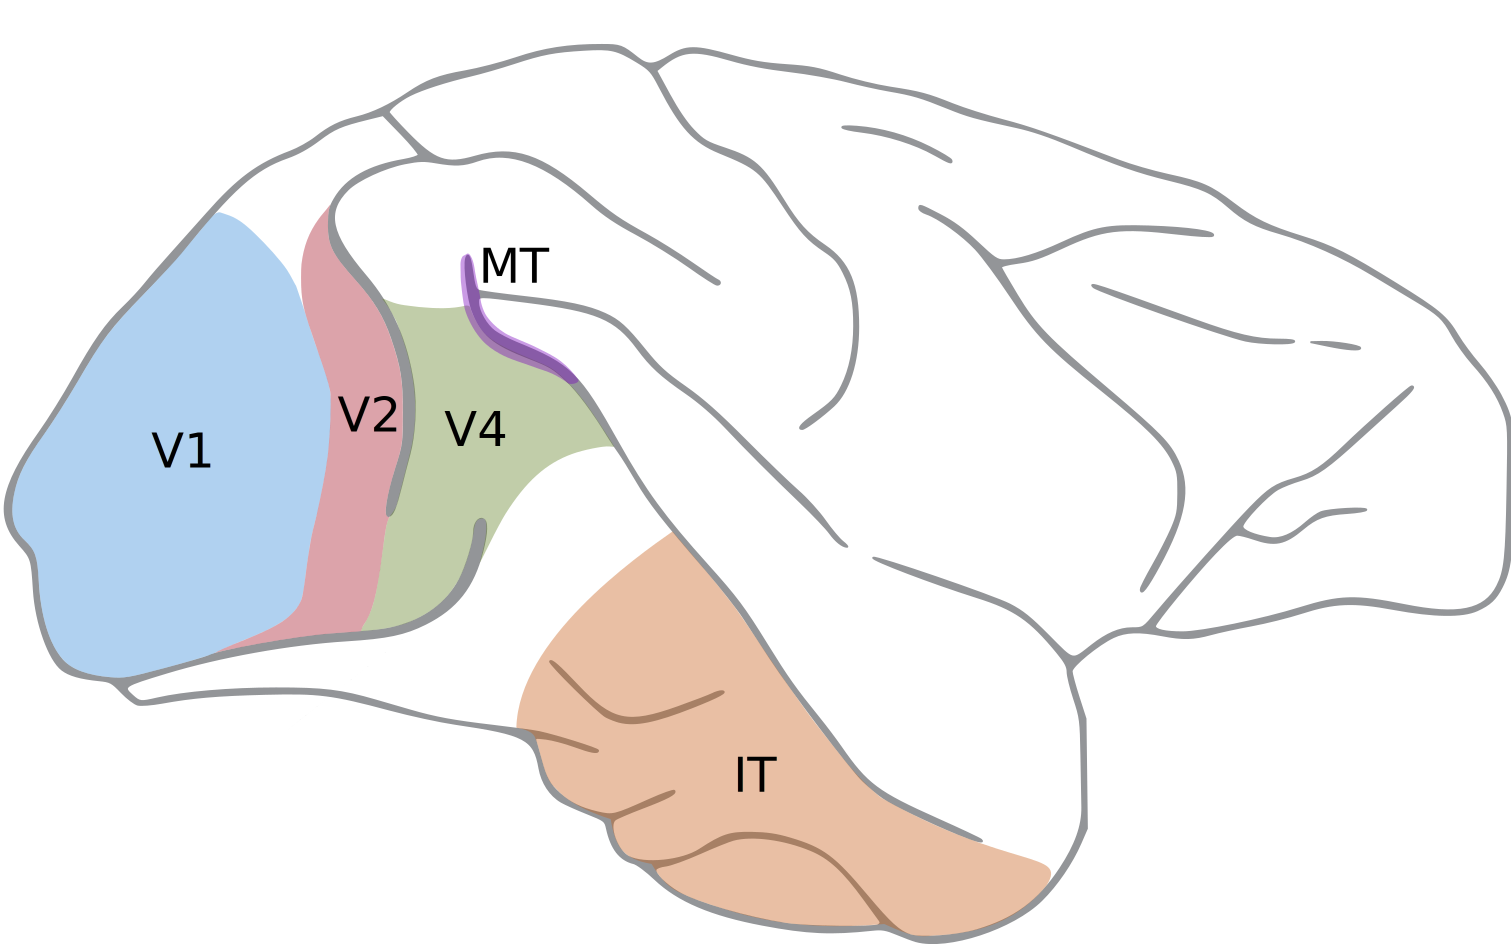
\includegraphics[width=86mm]{rhesusCerebrum.pdf}}
	\caption{\textit{The Rhesus Macaque Visual Hierarchy.} Each area depicted here is distinct in cytoarchitecture and maintains a complete retinotopic map. Information flows from the \gls{lgn} (not shown) to V1, then V2, V4, and finally the inferior temporal cortex (IT) in what we call the Ventral stream. }
	\label{fig:brain}
\end{figure}

It is known that each of these brain regions are unique and self-contained stages in hierarchical information processing. One reason they are thought to be unique stages is because each area has a full representation of the visual field (Retinotopic map) \citep{Felleman1997}. It has also been shown that neurons in these brain areas respond differently to the same visual information \citep{Mahon2001}, and have different functional architecture \citep{Yoshioka1996, Hubel1965}. At each stage of the hierarchy, the visual information is processed in increasingly complex ways. Information in photoreceptors is quite simple: it consists of how many photons of light there are at each point in the visual field. The \gls{rgcs} then sum that information and describe the first spatial derivative of the photoreceptors, where the changes in the concentration of light are (i.e. contrast edges; \cite{Wiesel1959}). The simplicity of this intra-areal computation is contrasted by the more intricate transformations between brain areas. For example, Hubel and Wiesel demonstrated that neurons in V1 respond dynamically to the orientation of a bar of light \citep{Hubel1959}, and so their firing rate contains information about orientation. Knowledge about the neural activity reduces the uncertainty about the stimulus and vice-versa. This stimulus-response relationship is the prototypical sensory coding function called a tuning curve. Studies have shown that the amount of stimulus information represented in the tuning curve of a neuron is highest at the peak (the stimulus that causes the highest firing rate) and the peak of the first derivative (largest slope), depending on the noise present in the system \cite{Butts2006}. Investigations into the neural code of the visual system therefore need to find stimulus dimensions that result in steep tuning curves and large peak responses from neurons. While bars of light are sufficient to investigate the neural code in early visual areas, these same stimuli are too impoverished to excite neurons in later areas. The low response rates are obstacles to describing the response function of neurons higher up in the visual hierarchy, like V4. The goal is still to find the domain in stimulus space that results in substantial, dynamic responses from a neuron, but the dimensionality of the stimulus space is astronomically larger. In the same manner that Hubel and Wiesel manipulated the width/orientation of a bar of light to excite V1 neurons, researchers have been developing novel strategies to make stimuli better suited for neurons in other visual areas \cite{Hubel1959, Pasupathy2002, Ponce2019, Cowley2017}. The resultant stimuli can be roughly categorized by the order of the underlying image statistics: first, second, and high-order. It is a precarious endeavor to match the complexity of a stimulus to the intricacy of a brain area's tuning preferences, but decades of work have guided a growing, cohesive understanding of stimulus-response functions. This work has lead to substantial improvements in sensory models of the brain as well as fundamental coding principles that generalize beyond the visual system.

%-----------------------------------
%	SUBSECTION 1
%-----------------------------------
\subsection{Subsection 1}



%----------------------------------------------------------------------------------------
%	SECTION 2
%----------------------------------------------------------------------------------------

\section{The Neural Response Function}
In its simplest form, one can consider visual neurons to be a biological implementation of some unknown function of a stimulus parameter ($\theta$):

\begin{equation}
R_n = f(\vec{\theta})
\end{equation}

%\begin{equation}
%f(\vec{\theta}) : \mathbb{R}^{n} \rightarrow \mathbb{R}
%\end{equation}

The neuron takes in inputs from dendrites, and produces an output in the form of action potentials (spikes). Computational neuroscientists then try to understand how the brain processes information by studying the input-output relationship of these functions. We begin with a single neuron, and a single variable input ($\theta$), to build the foundations for high-dimensional cases later.

\subsection{Tuning in One Dimension}

The prototypical representation of a neurons input-output function is the tuning curve. Tuning curves are estimated by taking discrete samples along a single feature dimension (orientation for example) and plotting the neural responses against the stimulus parameter (Figure \ref{fig:tuningIntro}A). In this case, each dot represents one trial of the stimulus-response function, and by averaging across trials we get an estimate (dotted line) of how a neuron responds to that stimulus dimension ($\theta$). This process provides the expected response of a neuron to each part of the stimulus space (Figure \ref{fig:tuningIntro}B) under the assumption that the tuning function is smooth where not sampled (\textbf{CITE FOR SMOOTH TUNING}). 
 
\begin{figure}[h]
	\centerline{\includegraphics[width=172mm]{tuningSamplingIntro.pdf}}
	\caption{\textit{Calculating a 1D Tuning Curve.} A.) The process for estimating a single neurons tuning curve to a single stimulus parameter $\theta$. Discrete stimulus values were chosen ($-180^\circ\ by\ 45^\circ\ to 180^\circ$) to span the stimulus space, and repeatedly presented (Gray dots). This provides the expected response to a given stimulus value (dotted line) for the neuron. B.) The estimated tuning and variability for the neuron in panel A.}
	\label{fig:tuningIntro}
\end{figure}

Importantly, this method also provides the reliability of the neural response function. While neurons are believed to respond in a deterministic manner, the presence of uncontrollable variables (biological noise \parencite{Faisal2008}, network oscillations \parencite{Fries2005}, latent factors \parencite{Yu2009, Chen2006}, etc.) makes most neurons appear to behave somewhat stochastically. That is, on any given trial, it may respond more or less than expected, which we call response variability. Tuning and variability both impact information signaling in unique ways, with different implications for the brain. 

A neurons tuning curve contains information. That is to say, knowledge of a neurons firing rate reduces uncertainty about the state of the world. Take the neuron from Figure \ref{fig:tuningIntro} for example. If the neuron is firing at $40\frac{spk}{s}$, it is pretty unlikely that the stimulus is either $0^\circ$ or $180^\circ$, so it is conveying information about the stimulus to other neurons. The question then becomes, \textit{how much} information a neuron is signaling. This quantity is directly related to three main components:

\begin{enumerate}
	\item Response Range
	\item Shape of tuning curve
	\item Response Variability
\end{enumerate}

The first point is addressed through natural upper and lower bounds. Neurons cannot have a negative firing rate, and neurons cannot fire arbitrarily fast due to biochemical constraints such as repolarization of chemical gradients and refractory periods (\cite{Kole2012}). The final two points are intertwined due to quantization of response and precision of readout. Neurons cannot fire half a spike, so a single neuron cannot encode to arbitrary precision (e.g. $45^\circ$ vs $45.000001^\circ$; remember that firing rates are bounded), even with 0 response variability. This makes properly utilizing the available range essential, i.e. the shape of the tuning curve.

\begin{figure}[h]
	\centerline{\includegraphics[width=172mm]{tuningAndInfo.pdf}}
	\caption{\textit{Tuning curves and Information.} A.) Von Mises tuning functions with different concentration parameters ($\kappa$). Color indicates highest information tuning functions for fine (Blue) and coarse (red) discrimination. B.) Mutual information (Firing Rate and orientation) as a function of $\kappa$. Blue line depicts $1^\circ$ discrimination, Red line depicts the more realistic situation of 8 stimulus classes ($0^\circ$ to $315^\circ$ in $45^\circ$ steps). }
	\label{fig:tuningInfo}
\end{figure}

Previous work has demonstrated that the most informative parts of a tuning curve is where the slope is highest \parencite{Series2004}. A small change in the stimulus results in the largest change in the response, making those sections the most sensitive to the stimulus dimension. Given this, one may fall into the trap of thinking larger slope means more information. Consider instead the black tuning curve in Figure \ref{fig:tuningInfo}A. If the task is to discriminate between $\theta=45^\circ$ and $\theta=90^\circ$, this is the worst stimulus-response function to use. In fact, the shape of a neurons tuning curve has been shown to vary with the demands on the system \parencite{Scott2023}. In the case of tuning width ($\kappa$ parameter of a Von-Mises function), course discrimination ($0^\circ$ vs. $45^\circ$) necessitates a wider tuning function than fine discrimination ($0^\circ vs. 1^\circ$; Figure \ref{fig:tuningInfo}B). This is because we are optimizing the tuning function for discrimination across the whole available range of $\theta$, not just the high-slope regions. 


%Neurons were modeled with an average response following \textbf{REFERENCE TO VON MISES EQUATION}. In this way, each stimulus value corresponds to an expected response (\textbf{LAMBDA}), which was then used as the rate parameter to pull trials from a poisson distribution.

\subsection{nD Stimulus Spaces: Multiple Features}
In the previous section I discussed the basics of tuning in 1 dimension. This explored how one neuron responds to changes in one stimulus parameter $\theta$. This is an oversimplification of the true process, as no true stimulus can be described with only a single number. In this section I will expand the concept of a 1D tuning curve to an nD tuning surface spanning multiple feature dimensions. 

\begin{figure}[ht]
	\centering{\includegraphics[width=172mm]{gabor2DStimSpace.pdf}}
	\caption{\textit{Gabors as points in a 2D Stimulus Space.} A.) examples of Gabor stimuli with various $\theta$ and spatial frequency values. B.) Positions of the Gabors depicted in panel A within a 2-Dimensional stimulus space. }
	\label{fig:gabor}
\end{figure}

One of the most heavily-studied and simplest stimuli used in studies of visual neuroscience is the Gabor (Figure \ref{fig:gabor}A). Gabors (or wavelets) are essentially oscillating light and dark patches at an orientation. These stimuli are often used in low-to-mid-level visual areas such as \gls{lgn} (\cite{Mahon2001}), V1 (\cite{Bredfeldt2002,Lennie1990, Tanigawa2010}), V2 (\cite{Gegenfurtner1996, Liu2020}) and \gls{mt} (\cite{Movshon1996, Rust2006}). Most such studies use the orientation dimension to produce tuning curves as described previously (Figure \ref{fig:tuningIntro}A), but many make necessary choices which limit them along non-studied feature dimensions (eg. spatial frequency, color, size, etc.). Let us begin with a 2D feature space by adding spatial frequency to orientation. Figure \ref{fig:gabor}A demonstrates how independently varying the two feature dimensions results in a set of stimuli that a particular neuron may be tuned for. These are of course discrete steps representing two continuous feature dimensions (orientation and spatial frequency). This results in an important conceptualization, the stimulus space (\ref{fig:gabor}B). Here, every possible combination of orientation and spatial frequency are represented as points in a plane. 

This is a natural progression from the 1-Dimensional orientation case shown before. All experiments investigating orientation tuning, necessarily limit stimuli along other dimensions. So while spatial frequency (for example) is kept constant in those experiments, neurons are likely still responding according to their n-dimensional tuning function. This results in a tuning surface (or tuning manifold in $>2$ dimensions), such as in figure \ref{fig:2Dtuning}. Here we have the same model neuron from \ref{fig:tuningIntro}, where it's tuning before was just a slice (gray plane) through some 2D surface.

\begin{figure}[h]
	\centering{\includegraphics[width=86mm]{2Dtuning.pdf}}
		\caption{\textit{Tuning along multiple Feature Dimensions.} A neurons tuning curve, in 2 dimensions becomes a tuning surface. Gray plane represents the spatial frequency value at which the tuning for $\theta$ matches figure \ref{fig:tuningIntro}.}
		\label{fig:2Dtuning}
\end{figure}

This idea of multidimensional tuning is more realistic, albeit more cumbersome. One of the biggest problems with studying neuron behavior this way is how intractable it is in 3+ dimensions. Take the 1D tuning curve in \ref{fig:tuningIntro}A. An experimenter must test the neural response function at several points to get an estimate of the tuning curve (in this case 8 orientations), because we do not know a priori which values along the stimulus dimension any one neuron is sensitive to. If, for example, we took the neuron from \ref{fig:tuningIntro}A and only sampled $\pm 90^\circ$, we would conclude that the neuron is not tuned to orientation. This is to say there is a minimum required sampling of each stimulus dimension we are interested in. Additionally, neurons often perform nonlinear operations \parencite{Carandini2012} so we must sample each relevant dimension independently. This means to get a meaningful tuning curve for an N-dimensional feature space requires around $8^n$ individual stimuli (assuming 8 sampled values for each dimension) sampled with repetition (5-10 trials each). So for a Gabor stimulus with feature parameters 1.) Orientation, 2.) Spatial Frequency, 3.) Color, 4.) Contrast, and 5.) Size, with the minimum 5 trials each, an experimenter would have to show $163,840$ stimuli in a single recording session. This is of course just for Gabors, one of the simplest visual stimuli. In more naturalistic settings, the number of feature dimensions could count in the hundreds. This problem motivates a more intelligent approach to searching for high dimensional feature tuning, which I will expand on in Chapter \ref{ch:optim}.


\subsection{nD Response Spaces: Multiple Neurons}

In the last section I built on the 1D neural response function by introducing the idea of multiple input dimensions: multiple features. In this section I will bring it back to 1 feature dimension, and discuss the implications of multiple response dimensions: multiple neurons.

Take again the example of neurons in V1 that are tuned for the orientation of a Gabor. This time we show a population of 8 neurons with equally-spaced preferences for $\theta$ (Figure \ref{fig:stateSpace}A). We can assume for the moment that each neuron independently contributes information about the value of $\theta$ with its' firing rate. A brain area or decoder with knowledge of all 8 neurons firing rates can accurately estimate $\theta$. For example, if neuron 1 has a low firing rate, and neuron 2 has a high firing rate, $\theta$ is most likely to be around $0^\circ$.

\begin{figure}[h]
	\centerline{\includegraphics[width=150mm]{stateSpace.pdf}}
	\caption{\textit{Population Codes} A.) Tuning curves for 8 homogenous model neurons along the orientation feature dimension. Color at the bottom represents the values of $\theta$. B.) A 2-Dimensional state space plotting the responses of neurons 1\&2 from panel A. Color represents the value of $\theta$ that lead to each pair of neural responses.  }
	\label{fig:stateSpace}
\end{figure}

This brings up another important concept that parallels the stimulus space from figure \ref{fig:gabor}B, the Neural state space \parencite{Paninski2010,Cross2021a}. A state space is a representation of neural data in which each dimension (or axis) is the firing rate of one neuron (Figure \ref{fig:stateSpace}B). We can then plot experimental variables (eg. stimulus features) according to the neural activity they elicited. In figure \ref{fig:stateSpace}B, $\theta$ is represented by color, and plotted according to the relative responses of neurons 1 and 2 from panel A. This plot also represents the simplest case of a 1-Dimensional response manifold \parencite{Kriegeskorte2021, Chung2018}. 

An important point to make here, as discussed in \textcite{Kriegeskorte2021}, is that tuning curves (Figure \ref{fig:stateSpace}A) determine the shape of the neural manifold (Figure \ref{fig:stateSpace}B), but not the other way around. Different sets of tuning curves are capable of generating the same manifold geometry. 


For example, if neuron 1\&2 from figure \ref{fig:stateSpace}A had the same tuning curve, adding neuron 2 provides no extra information. The fact that their preferences are offset is where the extra information comes from. This does not remain true when one considers response variability from before, as two identical neurons can provide multiple samples simultaneously (e.g. one neuron with two trials, or two identical neurons with one trial). 

Likewise, another major issue when expanding intuitions about tuning beyond a single neuron, are shared neural variability. When neurons co-vary together within stimulus condition, we call these noise correlations \parencite{Cohen2009, Ruff2016, Snyder2014, Moreno-Bote2014a}.


\subsection{Next Steps}
The bulk of this thesis resides in the final section of this introduction, comparing high dimensional neural and feature spaces. As discussed previously, many studies have looked into tuning of neural populations to single feature variables, and more still investigated individual neural tuning in multiple feature dimensions. Quite few have attempted to investigate both simultaneously, due again to intractability of the problem. 
In chapter \ref{ch:papernak}, I first discuss how even the simple case of neural tuning to one feature dimension is complicated by task demands and behavioral context. Then in chapter \ref{ch:optim} I expand on neural optimization techniques to elucidate tuning for multiple features from a population of neurons. I will also expand on how to interpret and analyzed such rich data using techniques such as \gls{cca} and \gls{dca} on simulated neural populations with known tuning parameters. Finally, in chapter \ref{ch:maps}, I apply all previous theory and techniques in a series of experiments aimed at deriving simultaneous understanding about both high-dimensional spaces. 








% Ch1. 1D tuning and context effects
% Chapter Template

\chapter{\color{RoyalBlue!50!black} Neuronal Modulation Depends on Context and Feature Tuning} % Main chapter title

\label{ch:papernak} % Change X to a consecutive number; for referencing this chapter elsewhere, use \ref{ChapterX}

%----------------------------------------------------------------------------------------
%	SECTION 1
%----------------------------------------------------------------------------------------

\section*{Introduction}
The \gls{mt} area of monkey cerebral cortex is a well-studied extrastriate visual area known to have robust selectivity for visual motion features \parencite{Britten1992, Born2005, Pasternak2020}. Motion signals represented by the activity of neurons in this area are important for making memory-guided comparisons about visual motion direction \parencite{Lui2011, Wimmer2016, Katz2016}. Lesions of this area impair the ability to report whether the motion direction of a stimulus matched a previous example or not \parencite{Rudolph1999a, Bisley2000a}; whereas electrical stimulation of this area can bias the behavior of an animal as though a particular direction of motion was seen when in fact no direction information had been present \parencite{ Bisley2001, Salzman1992, Salzman1990}. These findings indicate a key role for \gls{mt} in representing behaviorally-relevant visual motion information, and demonstrate that \gls{mt} has an important role in task-related perceptual decisions. One open question, however, is how behavioral goals impact the neural activity in area \gls{mt} during sensory (e.g., encoding/decoding of stimulus) and non-sensory (e.g., reward contingencies, decision making, etc.) periods of the task.

Area \gls{mt} acts in concert with another brain area, the \gls{pfc}, in order to do memory-guided comparisons of motion direction. \Gls{pfc} and \gls{mt} are reciprocally connected \parencite{Ungerleider1986, Barbas1988, Petrides2006}, and both are involved in memory-guided motion comparison tasks \parencite{Zaksas2006}. Neurons in \gls{pfc} contain direction information during motion discrimination tasks, but this selectivity is largely attenuated when animals do not have to make perceptual decisions, or when that information is not relevant to the task \parencite{Hussar2009, Hussar2012, Hussar2013}. Previous research has also found reduced trial-to-trial variability in \gls{pfc} with increased task demands \parencite{Hussar2010}, suggesting \gls{pfc} neurons may be recruited to support task performance when needed. Because of the interconnected structural and functional relationship between \gls{pfc} and \gls{mt}, such a change in trial-to-trial \gls{pfc} variability with task demands may be reflected in \gls{mt} dynamics and altered processing of stimulus information, but this hypothesis remains untested.

To investigate this question, we measured how activity in \gls{mt} covaried with the differing demands of an active task and a passive task that used physically identical stimuli. The active task consisted of two random dot motion stimuli separated by a delay, where subjects (Rhesus macaques; \textit{Macaca mulatta}) had to report whether or not the direction of motion in the first stimulus (``\sample") matched the second (``\test''). During the passive task, no perceptual decision was required, but the motion stimuli were the same. Thus, despite practically identical sensory conditions, the task demands during active and passive tasks were different. Thus, the active task can be parsed as a sequence of: stimulus encoding (S1), memory maintainance (delay period), recall and comparison (S2), and finally decision making (S2/post-S2). For sensory periods (S1/S2), We hypothesized that heightened task demands during the active task would be reflected in sharper tuning, reduced trial-to-trial variability, and/or modulation gain, in line with prior findings about selective attention to motion direction \parencite{Trujillo2004, Ponce-Alvarez2013, Cohen2008, Arandia-Romero2016}. For the more cognitive aspects of the task (working memory, S1/S2 comparison signals, decision making), we expected to find stronger comparison effects, signals differentiating ``same" and ``different" trials independent of motion direction, in the active task. 

We found that the effects of heightened task demands depended on the amount of task-relevant stimulus information (e.g. direction selectivity) neurons conveyed. Specifically, we found three distinct modulation profiles for stimulus processing between the active and passive tasks: information-enhanced, information-suppressed, and \mbox{information-consistent} neurons. Neurons signalling enhanced task-relevant stimulus information during the active task displayed sharper tuning, and a preferential reduction in trial-to-trial variability, but no effect on comparison signals. In contrast, information-suppressed neurons displayed a flattening of their tuning curves with no effect of task on trial-to-trial variability. The third subpopulation of neurons (information-consistent), while significantly tuned to motion direction, displayed only weak effects of task on tuning or variability. Instead, the suppressed and consistent groups showed task-dependent comparison signals comparing S1 and S2. These results suggest a division of labor in area \gls{mt}, separating sensory processing and cognitive effects of the task across distinct subpopulations of neurons.

\section*{Results}
Three adult male Rhesus macaques (\textit{Macaca mulatta)} performed delayed visual motion comparison tasks while we recorded neural activity in MT (Figure \ref{fig:fig1}A). In the active task, monkeys indicated whether a second stimulus (``\test'') had the same or a 90-degree different direction of motion than a first stimulus (``\sample'') by making a saccade to one of two choice dots. All three monkeys performed above chance in the active task (m201, 10 sessions: $77.79\% \pm 1.08\%$ accuracy, m202, 28 sessions: $81.63\% \pm 0.95\%$, m317, 16 sessions: $85.77\% \pm 1.36\%$ ; $mean \pm Std$). The passive task, except for a different fixation point shape, was identical up to the choice window, at which time no choice target stimuli were shown and no further action was required to receive reward (Figure \ref{fig:fig1}A). 

\begin{figure}
	\centerline{\includegraphics[width=172mm]{Figure1_taskEffects.pdf}}
	\caption{ \textit{Task design and task modulation of MT firing rates.} A. Trials consisted of a pre-stimulus fixation period, a first stimulus  (S1), followed by a 1.5 second delay, then a second stimulus (S2) and a post-S2 fixation period. After the post-S2 fixation period subjects were either rewarded (passive task) or had to report a decision with a saccade and rewarded after correct choices (active task). Stimuli moved in one of 8 directions ($0^\circ$, $45^\circ$, $90^\circ$, $135^\circ$, $180^\circ$, $225^\circ$, $270^\circ$, $315^\circ$) during S1, and then S2 was either in the same direction, or $90^\circ$ off of S1 (rotated left or right). B. PSTHs of an example neuron that was recorded in both tasks. Solid line represents the neuron’s response to its preferred motion direction while dashed lines indicate $180^\circ$ away from preferred (“anti-preferred”) C. Receptive fields (grey) of each simultaneously-recorded neuron from one example session, along with the location and size of the stimuli (red). Black curve corresponds to example neuron in B. Contours represent isointensity responses at $50\%$ of the peak response. }
	\captionsetup{singlelinecheck = false, font=footnotesize, labelsep=space, width=172mm}
	\label{fig:fig1}
\end{figure}

Neurons were recorded with receptive field centers of $10.55 \pm 0.77$ Degrees of visual angle eccentricity ($mean \pm SEM$ across all neurons from all sessions; Figure \ref{fig:fig1}C for example session). Neurons were included for analysis if: 1.) Their 50\% isointensity response field (see \hyperref[{sec:methods}]{Methods}) was at least 30\% covered by the stimuli, 2.) the subject did at least 10 trials in each direction condition, and 3.) they were confidently recorded across both tasks (see \hyperref[{sec:methods}]{Methods}). This resulted in 254 well-defined neurons included for analysis. 

We were interested in the impact of cognitive demands on \gls{mt} activity. Such demands varied over the course of a trial in the active task, including periods where stimuli were present (i.e., during \sample\ and \test) and also periods where stimuli were absent (i.e., pre-\sample, the delay, and post-\test). For example, prior to \sample, the animal should prepare cognitive resources in anticipation of the stimulus. Then, during \sample, the animal must process and store task-relevant information (motion direction). During the delay, this information must then be maintained in working memory and the appearance of \test\ may be anticipated. During \test, task-relevant information must again be encoded, the stored information about \sample\ retrieved, and a comparison judgement made. These dynamic task demands may result in varying effects on \gls{mt} activity across these different stages. We first describe the effect of task demands on motion-direction signalling by \gls{mt} activity during stimulus presentations (\sample\ and \test).
Second, we will describe effects of task demands on \gls{mt} activity when stimuli were absent. Third, we will describe effects of task demands on \gls{mt} activity during the comparison stage of the task (\test\ through decision).

\glsreset{mi}
\subsection*{Task effects in MT depend on neural tuning}
We hypothesized that the accuracy of motion direction encoding in \gls{mt} would improve when that information was task-relevant (i.e., in the active task compared to the passive task).
To test this, we measured the \gls{mi} between neural firing rates and the motion direction of \sample\ and \test. \Gls{mi} quantifies how much information about one signal is provided by another signal (and vice-versa), and takes into account both the tuning of neural responses with respect to a stimulus as well as trial-to-trial response variability (\cite{Hatsopoulos1998, QuianQuiroga2009}; see \hyperref[{sec:methods}]{Methods}).
Across all neurons in our sample, we found similar degrees of motion direction signalling in the active and passive tasks (Figure \ref{fig:MI}A). As \gls{mt} is a mid-level sensory area, this was unsurprising. 

\begin{figure}
	\centering
	\includegraphics[width=86mm]{ClusteringFigMatched.pdf}
	\caption[Unsupervised Clustering of neurons by Task-Effect]
	{{\it Motion Information Clustering.} A.) Time course of mutual information between matched neurons firing rates' and motion direction in the active and passive task. B.) Time series for active minus passive motion information (\gls{mi}) within neuron. Each row is a single neuron matched across task, and color represents the difference in information. See \hyperref[{sec:methods}]{Methods} for clustering algorithm. C.) Within-cluster averages from panel B.}
	\captionsetup{singlelinecheck = false, font=footnotesize, labelsep=space}
	\label{fig:MI}
\end{figure}

We hypothesized that changing task demands might be especially impactful on the activity of neurons that signal task-relevant information.
That is, switching from passive viewing to a task requiring judgment of motion direction might have a particularly strong effect on neurons strongly signaling motion direction compared to neurons that did not signal that information so strongly.
To test this hypothesis, we calculated the task effect of motion information for each neuron by subtracting the timeseries during the passive task from the active task. This provided a metric which quantifies, at each timepoint, how each neuron signals motion direction information differently across tasks (Figure \ref{fig:MI}B). We then clustered neurons according to the Pearson distances between these task effect time-courses (see \hyperref[{sec:methods}]{Methods}). We found 3 clusters to be the most parsimonious model, and hereby refer to them as suppressed, enhanced, and consistent groups (Figure \ref{fig:MI}B\&C), which describes the average task effect on direction information for neurons within each cluster.

% not sure how/if to include this information
%($1 Cluster: BIC=1.191, 2 Clusters: BIC=1.206, 3 Clusters: BIC=0.941, 4 Clusters: BIC=1.020, 5 Clusters: BIC=1.091$)

We found it interesting that a substantial group of neurons displayed a marked reduction in \gls{mi} during the active task (suppressed), as it represents a detriment in the population of neurons for direction coding. Taken together with the enhanced neurons, which followed the expected pattern of improved direction signalling, these results suggest that heightened task demands result in task-relevant information becoming disproportionately represented in a smaller number of highly-informative neurons.

%\subsection*{\color{rouge} Heightened Task Demands Flatten the Tuning Curves of Less-relevant Neurons}
\subsection*{Heightened Task Demands Differently Impact Tuning for Subpopulations of Neurons}
We found that mutual information between neuron firing rates and motion direction changed when motion direction was task-relevant (active task) compared to when it was not (passive task). Since \gls{mi} takes into account both stimulus tuning and trial-to-trial variability, the observed changes in \gls{mi} could be consistent with a change in tuning, a change in trial-to-trial variability, or a mixture of both. To better characterize the nature of the task-demand effects we found, we separately analyzed tuning and trial-to-trial variability for enhanced, suppressed, and consistent neuron groups.

\begin{figure}
	\centering
	\captionsetup{singlelinecheck = false, font=footnotesize, labelsep=space}
	\includegraphics[width=86mm]{tuningAndHFmatched.pdf}
	\caption{{\it Effects of task demands differed depending on how informative a neuron was about task-relevant information.} A.) Average Tuning Curves for information-enhanced neurons during the active (purple) and passive (green) tasks. Both curves contain the same neurons. Error bars are $\pm SEM$ across neurons.B-C.) Same as A for information-suppressed and consistent groups respectively. D.) Average trial-to-trial variability during S1 quantified with \gls{hf} (See \hyperref[{sec:methods}]{Methods}). E-F.) Same as panel D for information-suppressed neurons and consistent groups respectively. G.) Slope of a linear fit to enhanced neurons' firing rates vs time during a 1s interval before S2 onset in the Active vs Passive tasks. There was a significantly higher ramping during the active task (***: $p=5.66\cdot10^{-5}$, t-test). H-I.) Same as panel G for information suppressed (ns) and consistent (**: $p=0.0098$) groups respectively.}
	\label{fig:interaction}
\end{figure}

We tested for differences in tuning for each group by calculating the average firing rate for each neuron, and compared effects of task, direction condition, and stimulus (3-way ANOVA: Figure \ref{fig:interaction}A-C). The main effect of `stimulus' (S1 vs S2) was negligible for each group (enhanced: $p=0.238$; suppressed: $p=0.187$; consistent: $p=0.531$), so for visualization purposes we plotted S1, which unlike S2 does not have concurrent comparison processes. We found the expected pattern of tuning modulation for enhanced neurons, with gain around preferred direction and suppression to 180 degrees off preferred, supported by an interaction effect between task and direction ($p \approx 0$: Figure \ref{fig:interaction}A). In contrast, the information-suppressed group showed a reduction in response around their preferred stimulus in the active task (Figure \ref{fig:interaction}B). Interestingly, the consistent group shows a slight increase in response to anti-preferred motion (180deg off pref) which results in a flattening of their tuning curves (task effect: $p=0.005$). This means that during the active task, neurons that had suppressed or consistent information  had flatter (broader) tuning profiles, which in isolation would constitute a deficit to direction coding when that information is task-relevant.

\glsreset{hf}
\subsection*{Trial-to-Trial Response Variability is Modulated by task and Stimulus Features}
In addition to tuning, \gls{mi} also takes into consideration trial-to-trial variability in responses. we reasoned that the task effects on \gls{mi} may be partially due to altered variability of neural responses. To test this, we calculated the entropy of neural responses (separated again by task, motion direction, and stimulus, 3-way ANOVA) and normalized measurements relative to those of a simulated Poisson process matched for intensity (\gls{hf}; see \hyperref[{sec:methods}]{Methods}).

We found an overall reduction in \gls{hf} in the active task, relative to the passive task for information-enhanced neurons ($F=60.24, p \approx 0$; Figure \ref{fig:interaction}D). Additionally, all three classes of neurons had a reduction in trial-to-trial variability that was a function of motion direction (enhanced: $F=6.64$, $p \approx 0$; suppressed: $F=6.97$, $p \approx 0$; consistent: $F=2.07$, $p=0.044$; Figure \ref{fig:interaction}D-F). Neurons had the largest reduction in \gls{hf} to their preferred stimuli, with weaker effects as motion direction diverged from this direction. The preferential reduction in variability was strongest in the information-enhanced group, consistent with the improvement to both tuning and \gls{mi}. No active vs. passive task effect was found for the information-suppressed group, though they did still display an effect of motion direction on \gls{hf} that was consistent with the enhanced neurons. Information-consistent neurons showed a weak improvement in \gls{hf} that likely counteracted the weak detriment in tuning, resulting in the net zero change in motion direction information that classifies the group.

To summarize, all three groups of information-modulated neurons displayed different patterns of tuning and variability modulation, which further supports our hypothesis that these groups of neurons differently contribute to the task.


\subsection*{Task Demands Modulate MT Firing Rates During Non-stimulus Periods}
We next turned our attention to the effects of varying task demands on \gls{mt} activity during periods when dot motion stimuli were absent (pre-\sample, during the delay between \sample\ and \test, and post-\test). Because no stimuli were present, effects during these intervals would be due only to cognitive processes (e.g., anticipation of \sample\ or maintenance of memoranda during the delay).
The pre-S1 period was highly predictable in this task (1000ms post fixation), so we expected to see a gradual increase (``ramping'') of firing rate during this period, reflecting anticipation. We quantified pre-\sample\ ramping as the slope of a linear fit to FR vs. time during a one second window before \sample\ onset. We found a significant task effect of pre-\sample\ ramping only within the information enhanced group (T-test Passive minus Active slopes: $p=1.02\cdot 10^{-4}$).

Next we considered the delay period between \sample\ and \test. Because the timing of this delay was also highly predictable in our task (always 1.5 seconds), animals could anticipate the appearance of \test. We also found significant ramping during the delay period for enhanced neurons ($p=5.66\cdot10^{-5}$) and consistent neurons ($p=0.0098$), where both groups had higher delay ramping in the active task (Figure \ref{fig:interaction}G-I).  This increased ramping in the active task may reflect additional task demands related to the preparation of the \sample\ and \test\ comparison.
We also asked whether \gls{mt} activity might continue to be selective for the motion direction of \sample\ during the delay, which could be consistent with a working-memory-related maintenance process. However, we found that \gls{mi} between \gls{mt} activity and \sample\ motion direction rapidly fell to levels consistent with the null hypothesis after \sample\ offset, and this did not differ based on task demands (Figure \ref{fig:MI}A).

\subsection*{MT Activity is Affected by Cognitive Aspects of Memory-guided Visual Comparisons}
During \test\ of a given motion direction, our active task required subjects to make a saccade to the right if the direction of the preceding \sample\ was the same (``same trial''), and a saccade to the left if the direction of the preceding \sample\ was different (``different trial'').
It has previously been observed that \gls{mt} neurons' responses to physically identical \test\ stimuli differed whether they came from ``same'' or ``different'' trials, which we termed a ``comparison effect'' \parencite{Lui2011,Zaksas2006}. 
Here we ask: (1) are CEs different in the active versus the passive task (when no comparison is needed); and (2) is the task-modulation of CEs (if any) different across the three neuron groups (enhanced, suppressed, consistent)?

\begin{figure}
	\centerline{\includegraphics[width=86mm]{CEproportions.pdf}}
	\caption{\textit{Recruitment of MT neurons for cognitive aspects of the task} A.) Schematic of comparison effect analyses. Neurons were classified into groups according to their Pearson distance during S1 and the Delay. Comparison effects were then calculated from S2 onset up to the appearance of the choice targets. B.) Proportion of neurons within each information group with significant $S>D$ signal at some point during the CE window in panel A. C.) Same as panel B for $D>S$ neurons.}
	\label{fig:CEproportions}
\end{figure}

We calculated comparison effects as the area under the receiver operating characteristics curve (AUC) within direction condition during \test, between ``same'' and ``different'' trials (Figure \ref{fig:CEproportions}A). We expected that the cognitive effects of the task may run orthogonal to the sensory improvements (i.e. stronger comparison effects in non-enhanced groups), and this would be indicative of a division of labor. We indeed found that information-suppressed and consistent groups showed a significant increase in the number of $S>D$ neurons with no effect in the information-enhanced group (Figure \ref{fig:CEproportions}B; Suppressed: $\chi^2=8.79, p=0.003$, Consistent: $\chi^2=4.05, p=0.044$). Interestingly, the suppressed group show a reduction in $D>S$ neurons in the active task (Figure \ref{fig:CEproportions}C; Suppressed: $\chi^2=8.53, p=0.0035$). An important point to note here, is that the same proportion of significant neurons in all three information groups shows CEs during the passive task, and the active task influenced their cognitive contributions differently. 

\begin{figure}	
	\centering
	\includegraphics[width=86mm]{CEtimecourses.pdf}
	\caption{\textit{Comparison Effects increase from stimulus to decision} A.) Time course of comparison effects (AUC between same and different trials within stimulus type) for neurons that were information-enhanced and significantly $S>D$ in either task. B.) Same as panel A but for information-enhanced $D>S$ neurons. C-D.) Same as A-B but for information-suppressed neurons. E-F.) Same as A-B but for information-consistent neurons. *: $p<0.05$ for the difference between tasks over the indicated interval.}
	\label{fig:CEtimecourses}
\end{figure}

We next looked at the time courses of comparison effects from S2 through appearance of the choice dots (Figure \ref{fig:CEtimecourses}), again separated by information-group and direction of CE. These time courses reflect the aforementioned division of labor, where the information-suppressed and consistent groups contribute to the cognitive aspects of the memory-guided comparison (Figure \ref{fig:CEtimecourses}C-F), while the information-enhanced group does not (\ref{fig:CEtimecourses}A-B). So, in addition to a higher proportion of neurons signalling CEs, the average CE signal ($S>D$) during the post-S2 window also increased with heightened task demands (Figure \ref{fig:CEtimecourses}C \kst\ test: $p=1.11 \cdot 10^{-5}$; Figure \ref{fig:CEtimecourses}E \kst\ test: $p=8.22 \cdot 10^{-4}$). The higher proportion of $S>D$ neurons in the suppressed and consistent groups, along with their increased CE signalling, indicates that while these groups did not improve stimulus encoding with heightened task demands, they were recruited to aid with the comparison of S1 and S2. 


\section*{Discussion}
\glsresetall
We hypothesized that neurons in the primate \gls{mt} area behave differently when task demands increase in order to improve information processing for goal-oriented behavior. We tested this hypothesis by recording activity of \gls{mt} neurons in monkeys performing two tasks, one active and one passive.
We found that in the active compared to the passive task, (1) three patterns of task effects on information signalling arose that were distributed across subpopulations of neurons, and (2) sensory and cognitive aspects of the tasks are handled separately by these subpopulations.

We found that firing rates of neurons in \gls{mt} contained direction information during the stimulus periods (Figure \ref{fig:MI}A), and that increasing task demands had one of three broad effects on motion information for each neuron: information-enhancement, information-suppression, or information-consistent effects (Figure \ref{fig:MI}B). We then asked whether the changes in \gls{mi} were caused by tuning or variability. However, the extent to which tuning and variability are each influenced by cognitive factors has been a subject of intense research \parencite{Renart2014,Gilbert2013}, and each has different implications for computation and neural mechanisms. To better characterize the role of task demands on motion direction signaling in \gls{mt} in the context of this prior work, we separately examined tuning and variability. As the neurons were matched across task, we could directly compare how each neuron responded to motion in the active and passive conditions. Information-enhanced neurons showed sharper tuning curves with larger responses to their preferred motion direction and a suppression to anti-preferred (Figure \ref{fig:interaction}A). Information-suppressed neurons on the other hand, displayed a marked reduction in response to their preferred stimulus in the active task, resulting in the detriment to \gls{mi} observed. As a result, these neurons became less tuned for motion direction when that information was more task-relevant. These effects on tuning are consistent with the classification of neurons based on changes to motion direction signalling in \gls{mi}, but may not account for the full picture, as \gls{mi} is also affected by trial-to-trial response variability, which we examined next. 

By measuring \gls{hf}, we found a strong relationship between direction preference and variability, which did not depend on group (Figure \ref{fig:interaction}D-F). Neurons had the largest reduction in trial-to-trial variability during presentations of their preferred stimulus, with weaker effects as direction diverged from preferred. This cannot be due to the increased firing rate for those directions, as \gls{hf} accounts for rate effects (see section \hyperref[{sec:methods}]{Methods}), and a rate confound would result in the opposite trend (that is, typically variability is biased downward for lower rates, but we found higher variability at lower rates; \cite{Churchland2010}). The effect of heightened task-demands in the active task was largest for the information-enhanced neurons, which compound the tuning-based improvements to \gls{mi} (Figure \ref{fig:interaction}D). Interestingly, suppressed neurons showed no effect of task on variability, whilst maintaining the effect of motion direction. This means that heightened task demands flatten the tuning curves of these neurons, without altering the trial-to-trial variability.
Previous researchers have suggested that a substantial portion of trial-to-trial variability can be understood in terms of neurons' susceptibility to changes in cognitive state \parencite{Ecker2016a,Denfield2018a}; thus one interpretation of this pattern of results is that these neurons decrease their participation in sensory processes (reduced tuning) while maintaining their participation in more cognitive processes (consistent trial-to-trial variability)
The reduction in trial-to-trial stimulus response variability we observed in enhanced neurons when task demands were elevated is reminiscent of the finding of \textcite{Mitchell2007}, who found general reductions in Fano Factor in V4 responses when animals selectively attended to a stimulus compared to when that stimulus was not attended.
The novel and more surprising result we found is that the strength of variability reduction depended on whether the stimulus was preferred (great reduction in variability) or less-preferred (less reduction in variability). This suggests that one effect of elevating task demands is a preferential improvement to information transmission reliability according to neurons' feature tuning.

We found significant changes in non-stimulus firing rate (FR) in the active task compared to the passive task, such as larger FR ramping during the delay period (Figure \ref{fig:interaction}G-I). Ramping of neural firing rates has traditionally been explored in the context of motor preparation \parencite{Ding2015, Narayanan2016}, and decision making \parencite{Shadlen2001}, where it has been typically linked to anticipation. Finding anticipatory increases in firing rate for sensory neurons in MT is interesting, and is not likely explained during the pre-\test\ interval of our tasks through either decision making or motor planning, as neither a correct decision or appropriate motor plan can be made before first seeing \test . 
More likely, the ramping we observed is related to preparing cognitive and attentional resources for the perceptual phases of the task, which had highly predictable timing, as has also been found for LPFC neurons \parencite{Hussar2010, Bisley2004}. This line of thought has also been explored in the context of another nearby visual region, V4 \parencite{Snyder2018,Luck1997}, where anticipatory ramping has been linked to interactions between V4 and prefrontal cortex \parencite{Snyder2021}. 
Taken together, these results suggest anticipatory signals may originate in prefrontal cortex and influence visual cortex via top-down feedback.

In addition to the more strictly sensory aspects of the task, the active task contains a comparison component which requires additional cognitive resources such as working memory. 
A greater response to \test\ on ``different'' trials compared to same trials (``$D>S$'') could be consistent with a response adaptation effect, while a greater response to \test\ on ``same'' trials (``$S>D$'') would be more consistent with a facilitation effect \parencite{Kohn2003}. We would expect that if CEs in \gls{mt} are explained primarily by adaptation/facilitation, we should find similar effects in the active and passive tasks; any task effect should indicate a greater role for memory-guided comparison processes.
We found no difference in comparison effects for information-enhanced neurons but significantly more extreme comparison effects for the suppressed and consistent groups (Figure \ref{fig:CEtimecourses}).
These cognitive effects being isolated to neurons that became worse at signalling motion direction when that information became more task-relevant further supports a division of labor in area MT for completing the task.
We found that comparison effects emerged most clearly during the period after the offset of \test\ and before the execution of the response saccade (the `post-\test' interval). 
This underscores the non-sensory, cognitive nature of these effects (since the sensory stimulus was absent when effects were strongest), and reduces the potential that response adaptation or repetition suppression could explain D$>$S comparison effects \parencite{Lui2011,Kohn2003}.
This relatively late time-course of comparison effects in \gls{mt} differs from earlier reports, which found comparison effects emerging shortly after \test-onset \parencite{Lui2011,Zaksas2006}. 
One reasonable explanation for this difference in the timing of comparison effects across studies is the difference in timing between the onset of \test\ and the animals' reports. 
Earlier studies required the animals to respond immediately following the offset of the \test, whereas in the current study animals must withhold responding until after the post-\test\ delay. 
Thus, if the timing of comparison effects was more tightly related to the animals' reports than to the time of \test\ onset, then that would be consistent with the results across all these studies of comparison effects in \gls{mt} and further underscores the cognitive role of comparison signals.
Finally, in earlier studies decisions were reported with a manual button press \parencite{Lui2011,Zaksas2006}, whereas the current study required animals to report with a saccade, reinforcing the notion that comparison effects are related to cognitive decisions rather than the formation of particular motor plans.
\begin{center}
	\begin{table*}
		\begin{tabular}{|c|c|c|c|c|c|c|c|c|}
			\hline
			\textbf{Class} & \multicolumn{3}{|c|}{\textbf{Tuning}} & \multicolumn{3}{|c|}{\textbf{HF}} & \textbf{Delay Ramping} & \textbf{CE} \\
			\cline{2-7}
			& Task & Dir. & Stim. & Task & Dir. & Stim. &  &  \\
			\hline
			\textbf{\textcolor{enhanced}{Enhanced}} & *** & *** & ns  & *** & *** & * & *** & ns \\
			\textbf{\textcolor{suppressed}{Suppressed}} & *** & *** & ns & ns & ** & * & ns & ** \\
			\textbf{Consistent} & ** & *** & ns & ** & * & * & ** & * \\
			\hline
		\end{tabular}
		\caption{Task effects summary. Significance of task effects separated by information clusters (*: $p<0.05$, **: $p<0.01$, ***: $p<0.0001$, ns: not significant). Statistics for Tuning and entropy (HF) were a three-way anova between task, motion direction, and stimulus (S1 vs. S2). Comparison Effects (CE) were $\chi^2$ tests between the active and passive tasks (\ref{fig:CEproportions}B). Delay ramping was compared using t-tests on the slopes (Passive minus active: (\ref{fig:interaction} G-I).}
	\end{table*}
\end{center}

\subsection*{Conclusion}
In the present study, we investigated the effects of task demands on information processing in area MT of the macaque. We found substantial differences in variability and tuning profiles depending on the degree to which a neuron represented task-relevant information in its firing rate. In addition to these sensory components of the task, MT neurons also show stronger cognitive signalling with heightened task demands, such as anticipatory ramping and heightened comparison effects. These results highlight the role of MT populations in all phases of memory-guided comparisons of visual motion direction, and, combined with the previous findings in \gls{pfc}, suggest a continual interplay between prefrontal and extrastriate visual cortical areas during cognitive task performance. Importantly, involvement in sensory versus cognitive processes was found to be flexibly distributed across subpopulations of \gls{mt} neurons, with some neurons taking on greater sensory signaling when task-relevant, and other neurons shedding sensory selectivity in seeming favor of greater cognitive responsibilities.



\section*{Methods}
\label{sec:methods}

\subsection*{Resource Availability}
\subsubsection*{Lead Contact }
Requests for further information should be directed to the lead contact Adam Snyder (adam.snyder@rochester.edu).

\subsubsection*{Materials Availability }
This study did not generate any new reagents. 

\subsubsection*{Data and Code Availability}
Data and code used for this paper are made available by request through the lead contact.

\subsection*{Subjects} 
Subjects used in this study were three adult male rhesus macaques ages 7, 8, and 7 years, for 201, 202, and 317. All training, surgery, and experimental procedures were performed in accordance with the National Institutes of Health \textit{Guide for the Care and Use of Laboratory Animals} and were approved by the University of Rochester Committee for Animal Research. Surgery was performed using aseptic technique with isofluorane general anesthesia and perioperative opiate analgesics. An initial surgery was performed to implant a surgical steel head holder restraint embedded in bone cement secured to the cranium with ceramic bone screws. After behavioral training, a subsequent surgery was performed to implant a PEAK canula (19 mm diameter; Crist Instruments, Hagerstown, MD) over MT.

\subsection*{Data Acquisition} 
Recording chambers enclosed the craniotomies and contained 1mm-spaced CILUX grids (Crist Instruments). Thirty-two-channel S-probes (Plexon, Dallas Texas) were lowered through custom-made steel guide tubes, which were themselves inserted just low enough to penetrate the dura. We then drove the electrodes using a NAN electrode drive (NAN Instruments, Nof Hagalil, Israel). Recordings were done by coordinating a Plexon (Dallas, Texas) Multichannel Acquisition Processor and the data acquisition system TEMPO (Reflective Computing).

\subsection*{Receptive Field Mapping}
Prior to each recording session, receptive fields were mapped in order to identify where the stimuli should be displayed. The initial manual phase consisted of moving a patch of dot motion around on the stimulus display with a computer mouse while listening to spiking activity via an audio monitor. Afterwards, we presented small dot motion patches ($1^{\circ}$) in different directions on the vertices of a grid spanning the likely RF area identified in the manual step. Stimuli for each session were placed such that they covered the aggregate receptive field area for the recording (Figure \ref{fig:fig1}B).

\subsection*{Stimulus Presentation}
Stimuli were presented at 75 Hz monitor refresh rate on a 19-inch IIyama Vision Master Pro-513 monitor with 1,152 by 870 pixel resolution. They were $100\%$ motion-coherence random dot kinematograms in one of 8 directions ($0^\circ, 45^\circ, 90^\circ, 135^\circ, 180^\circ, 225^\circ, 270^\circ, 315^\circ$) placed in a circular aperture fit to the size of the receptive fields, with a dot diameter of $0.03^{\circ}$ and a density of 3$\frac{dots}{deg^2}$. Dot luminance was 15$\frac{cd}{m^2}$, shown on a dark background of 0.1$\frac{cd}{m^2}$. Monkeys were required to maintain fixation within $2^{\circ}$ of a central dot throughout the trial until the response interval, and eye position was monitored with an ISCAN infrared eye-tracking device.

\subsection*{Task Design}
Trials started once subjects fixated on a central dot. They then had to maintain fixation for 1 second before \sample\ onset. Both \sample\ and \test\ lasted 500ms. \sample\ was followed by a 1.5 second delay period, and then the second stimulus \test\ was presented. Subjects then had to wait an additional 1s after \test\ offset before either a choice was required (active task), or they were simply rewarded (passive task). For the active task, the central fixation point was extinguished at the beginning of the response interval, and two identical choice targets were presented 5 degrees to the right and left of fixation, and the animal indicated its judgement as to whether \sample\ and \test\ were the same direction or not by making a saccade to the right or left choice target, respectively. In most recording sessions, we collected data for both the active and the passive tasks. We always collected data for the active task before the passive task, because animals would have been unmotivated to perform the more difficult active task if they had performed the easier passive task first.

\subsection*{Data Analysis} 
Spike sorting was done offline with Plexon sorter (Version 3.3.2) by using \gls{pca} on the spike waveforms and manually clustering. A neuron was included for analyses if there were at least ten trials in each direction condition, and if the stimuli covered at least 30\% of its 50\% isointensity response field. A total of 1264 neurons across both tasks passed these criteria (201: n = 263, 202: n = 454, 317: n = 547), with 928 neurons recorded in the active task and 336 neurons recorded in the passive task. Of those neurons, 254 were confidently matched across task and included for further analysis. Neurons were considered matched across task if they were recorded on the same channel and their waveforms were highly correlated ($R^2>0.99$). All subsequent analyses were done using custom routines for Matlab 2020a (The MathWorks, Inc, Natick, MA).

\glsreset{mi}
\subsection*{Mutual Information} 
\Gls{mi} quantifies information (in bit) shared between two variables, i.e.: how much the uncertainty about one variable (motion direction condition, in our case) may be reduced with knowledge about the second variable (spike counts). \Gls{mi} provides a robust metric of direction selectivity that accounts for changes in tuning curves, variability, and absolute firing rates. We calculated \gls{mi} using:

\begin{equation}
MI(x,y)= \sum_x \sum_y p(x,y) \log_2\left(\frac{p(x,y)}{p(x) p(y)}\right)
\end{equation}

Where $p(x,y)$ is the joint probability distribution between number of spikes and direction condition, and $p(x) p(y)$ is the product of marginal probability distributions. 
This provides how many bits of information a neuron's firing rate contains about direction and vise versa. 
For $p(x)$, we used the probability of observing a spike count in a bin of width $\Delta x$ sp/s, where the bin width was determined by ``Scott's rule'' \parencite{scottsRule}:

\begin{equation}\label{eq:spikebin}
\Delta x = \frac{3.5 n^{-\frac{1}{3}}}{n} \sum_{i}^{n}\left( x_i-\bar{x} \right)
\end{equation}

We calculated the mutual information between spike count and \sample\ direction for each non-overlapping 50ms bin from the start of each trial up to the end of the delay, and then the MI between spike count and \test\ direction through the end of the trial. In order to correct for spurious effects that come from differences in trial-counts, we baseline-corrected \gls{mi} by calculating it many times with shuffled conditions, and subtracted this out \parencite{Hatsopoulos1998}. We then computed the bitrate by dividing this metric with the bin size (0.05s).

\begin{equation}
I(x;y) = \frac{MI(X;Y)- MI_\textrm{shuffled}(X;Y)}{0.05s}
\end{equation}


\glsreset{mi}
\subsection*{Classification of neurons into information Enhanced, Suppressed, and Consistent subgroups}
We calculated baseline-corrected \gls{mi} between the firing rate of a neuron and motion direction shown for each time bin. From trial start through S2 onset \gls{mi} was calculated according to S1 direction. From S2 onset through the end of the trial, it was calculated between firing rate and S2 direction. 

We then took the \gls{mi} time series for a neuron in active, minus passive, in order to get a task-effect of motion information over time. Note that this was only possible for neurons that were successfully matched across tasks (n=254). The clustering algorithm contains 3 distinct steps.\\

1.) Calculate the Pearson distance (i.e., one minus the Pearson correlation) between each pair of neurons' task-effect time series. This was done on a window from trial start through the end of the delay. We did this in order to disentangle the sensory and cognitive components, since clustering on S2 would create a circularity for later analyses. \\

2.) Reduce the dimensionality with multidimensional scaling to five dimensions (to mitigate the ``curse of dimensionality'' for clustering with high-dimensional data).\\

3.) Model selection to pick the appropriate number of clusters. This consisted of fitting multiple Gaussian mixture models to the data, each with different numbers of components. We then selected the appropriate number of clusters by selecting the model with the lowest Bayes Information Criterion (BIC), which was three clusters.\\

4.) K-means clustering using the appropriate number of components (3) determined in step 3. 

In this way, neurons were partitioned into groups based on how motion information signalling changed across the active and passive tasks. This allows us to then see how other task-related effects may depend on the type of information modulation a neuron receives.

\subsection*{Entropy Factor} 
Entropy Factor (HF) quantifies the entropy of a neuron's spike count (across trials) relative to a Poisson process with the same rate parameter, $\lambda$ \parencite{Rajdl2017}. It is similar to Fano factor, in that a value of 1 indicates equivalence to a Poisson process, while values greater or less than 1 indicate distributions that are supra-poisson or sub-poisson, respectively. However, unlike Fano factor, which compares the variance of a distribution of spike counts to its mean, entropy factor takes into account the entire distribution of spike counts. This provides a more reliable metric than Fano Factor, particularly when there are a low number of observations, for which sample variance is biased lower than the expected variance in the limit of infinite data. For each 50ms time bin, $t$, we calculated the entropy $H_{Observed}(\harpoon x_t)$ of the distribution of spike counts ($\harpoon x_t$) across trials with the same stimulus direction and divided it by the entropy of a simulated Poisson distribution with the same intensity and number of trials.

\begin{equation}
HF(\harpoon x_t) = \frac{H_{Observed}(\harpoon x_t)}{H_{Poisson}( \hat{x})}
\end{equation}

Here, $H_{Observed}(\harpoon x_t)$ is the entropy of the distribution of spike counts across trials $i \in [1,n]$ for a neuron at time $t$, defined by:

\begin{equation}
H_{Observed}(\harpoon x_t) = - \sum_{i=1}^n{p(x_t^i) \log\left(p(x_t^i)\right)}
\end{equation}

\noindent where $H_{Poisson}(\hat{x})$ is the entropy of a simulated Poisson process with rate parameter $\lambda$:

\begin{equation}
%    \lambda = \frac{1}{n} \sum_{i=1}^n{x_t^i}
\lambda = \bar{x}_t
\end{equation}

The entropy of a Poisson process was calculated by doing 200 simulations of spike counts for $n$ trials pulled from a Poisson distribution with rate parameter $\lambda _t$, and the same unbiased bins used for the data (eq. \ref{eq:spikebin}. By then averaging the observed entropies of the simulations, we get an estimate of how variable, on average, we would expect the matched Poisson process to be. This normalization accounts for bias in sample entropy due to differences in firing rate or trial count. 

\subsection*{Tuning Curves}
Tuning curves were calculated as the average firing rate during the stimulus window for each of the 8 directions. For testing the effect of stimulus (S1 vs. S2) on tuning and HF, we used a three-way ANOVA with factors of `direction' (eight levels corresponding to each motion direction), `stimulus' (two levels: S1 vs. S2) and `task' (two levels: active vs. passive).


\subsection*{Comparison Effects}
Comparison effects (CE) were calculated as the area under the curve of the Receiver Operating characteristic (AUC). For each neuron, trials were separated by direction condition (during S2), and then by trial type (same direction or different direction trials depending on whether S1 matched S2). CE was calculated on firing rates (convolved with a 100ms smoothing kernel) for each non-overlapping 10ms bin, as the AUC between `same' trials and `different' trials within direction. AUC values were then averaged across direction condition within each time bin, resulting in a time course of AUC values for each neuron. Values greater than $0.5$ indicates a neuron that responds more robustly to identical visual stimuli on trials where the directions of S1 and S2 matched ($S>D$ neurons), while values less than 0.5 indicated the opposite ($D>S$ neurons). 

\subsubsection*{Statistical Significance of CE}
Statistical significance of CE was determined using a bootstrapping procedure. Trial labels (`same' or `different' trial) were randomly permuted, and AUC values were calculated 500 times per neuron. A neuron was considered significantly CE signalling (Figure \ref{fig:CEproportions}) if its AUC was significantly different from the bootstrap distribution ($\alpha=0.025$: two-tailed) for a significant number of time-points ($\alpha=0.05$: one-tailed). That is, the CE signal was stronger than expected by chance for a longer period of time than expected by chance. Observed CE values greater than the bootstrap distribution is same-preferring ($S>D$) and lesser than the bootstrap distribution is different-preferring ($D>S$).

For comparing the magnitude of CE over time for neurons significantly CE-signalling (Figure \ref{fig:CEtimecourses}), we averaged the CE values over two time windows of interest: the S2 period (0 to 500 ms relative to S2 onset) and the post-S2 period (500 ms to 1.5 s relative to S2 onset).
We then tested for the difference in CE between tasks for each group of neurons (enhanced, suppressed, consistent) for each type of comparison signal ($S>D$, $D>S$) and for each time window of interest using a \kst\ with $p<0.05$ (Bonferroni-corrected for the twelve repeated tests) considered significant.

% Ch2. stimulus optimization for neural populations (simulations)
% Chapter 1

\chapter{Stimulus Optimization for Neural Populations} % Main chapter title

\label{ch:optim} % For referencing the chapter elsewhere, use \ref{Chapter1} 

%----------------------------------------------------------------------------------------

% Define some commands to keep the formatting separated from the content 
\newcommand{\keyword}[1]{\textbf{#1}}


%------------------------------------------------------------------------------------

\section{Optimization}
Consider here, \textbf{EXAMPLE OF EASILY-UNDERSTANDIBLE OPTIMIZATION PROBLEM}. This example demonstrates that optimization, at the outset, is a simple problem. The complexity comes from large, high-dimensional data sets, and the plethora of approaches available. In this chapter, I will first describe the two main classes of optimization. Second, I will link these concepts to functional properties of neurons, focusing heavily on the visual system. I will then compare multiple algorithms when optimizing simulated neural data. 
\subsection*{What is Optimization?}
In its simplest form, optimization begins with an unknown function of inputs $\vec{x}$:
\begin{equation}
	f(\vec{x}) : \mathbb{R}^{n} \rightarrow \mathbb{R}
\end{equation}
where the output of the function is deterministic of it's inputs $\vec{x}$. The goal of optimization is to then find the set of inputs which minimizes (or maximizes) the output of the function $f(\vec{x})$. \textbf{MORE INTRO TO THIS SECTION BEFORE DERIVATIVES}

\subsection{Derivative-Based Optimization}
\label{sec:DerivB}
\textbf{MORE INTRO TO THIS SUBSECTION}
We an illustrate this using the simple example of a parabola. 
\begin{figure}
	\centering
	\includegraphics[width=86mm]{parabolaGradient.pdf}
	\caption{\textit{FigureTitle}}
	\label{fig:parabolaGradient}
\end{figure}
In the realm of low-noise and few variables, optimization is a rather simple problem of calculating the gradient and following it (Figure \ref{fig:parabolaGradient}). In Figure \ref{fig:parabolaGradient}, we test the function by using two random inputs (points 1\&2), calculate the gradient (3), and follow the gradient for the next input (4). This is an iterative process whereby each time we sample the function, we obtain more knowledge about it. Continuing this process will eventually result in $x=2$ as the global minimum. While this may appear obvious, in real world problems the blue line is unknown, necessitating the use of optimization techniques.
Unfortunately, because data is often high-noise and high-dimensional (in the parabola example there is only one input $x$, but most problems have many), calculating gradients quickly becomes computationally intractable in finite time. In addition to these constraints, real-world problems are often non-convex, meaning they have many local minima where gradient descent fails (\textbf{MAYBE NON-CONVEX FIGURE EXAMPLE}). This problem belies standard gradient approaches and lead to the development of Derivative-Free optimization techniques (see \ref{sec:DerivF}).

\subsection{Derivative-Free Optimization}
\label{sec:DerivF}
\subsection{Manifold Approximation with Particle Swarm (MAPS)}
\subsection{Genetic Algorithm}
genetic algorithm doesn't explore the radial dimension well. Even with a-priori knowledge of the proper radius, it doesn't do any better than MAPS because of this (prove it?).
\subsection{Bayesian estimation of true gradients?}
\subsection{Comparison across algorithms}

\section{Simulated Neural Population}
Assumptions:
\begin{enumerate}
	\item Peak FR$= 100 \frac{spk}{s}$
	\item Independent tuning to each feature dimension
	\item Deterministic responses (could fix)
	\item Independent Neurons
	\item Ground truth stimulus
\end{enumerate}

$x-pref$ is a matrix of euclidean distances for the current stimulus to each individual neurons' preferred stimulus. tuning is the neurons covariance matrix for the latent space (nLatents x nLatents). Diagonal is tuning width in that dimension and 0s off diagonal because feature tuning is assumed independent
\begin{equation}
someSymbol = -(x-pref)^T * tuning * (x-pref)
\end{equation}

response function: (come up with symbols for terms)
\begin{equation}
	\harpoon y = Peak * \exp{}
\end{equation}



%------------------------------------------------------------------------------------


 


% Ch3. Tuning for Image statistics in V4/V1 (MAPS)
% Chapter 

\chapter{\color{thesisBlue} Using Generative Models of Natural Images to Define Neural Tuning Manifolds} % Main chapter title

\label{ch:maps} % For referencing the chapter elsewhere, use \ref{ch:maps} 

%----------------------------------------------------------------------------------------

% Define some commands to keep the formatting separated from the content 
%\newcommand{\keyword}[1]{\textbf{#1}}

%------------------------------------------------------------------------------------


%Investigations into sensory coding in the visual system have typically relied on the use of either simple, unnatural visual stimuli, or natural images. Simple stimuli, such as gabors, have been effective when looking at single neurons in early visual areas such as V1, but seldom produce large responses from mid-level visual neurons or neural populations with diverse tuning. Many types of ``Naturalistic" image models have been developed recently which bridge the gap between overly-simple stimuli and experimentally infeasible natural images. These stimuli can vary along a large number of feature dimensions, introducing new challenges when trying to map those features to neural activity. We propose a method that searches high-dimensional stimulus spaces for neural tuning in a closed-loop experimental design. Stimuli are generated in each block by using neural responses to previous stimuli to make predictions about the relationship between the stimulus space and neural response space. We found that these variables contained stronger linear relationships with neural activity than many other forms of image processing, including fourier decomposition or image compression in pixel space.


\section{Introduction}
Research into sensory coding in the visual system focuses on determining what visual features neuronal activity covaries with, i.e. what information is it encoding. Traditional experiments looked at neural responses to simple stimuli such as small patches of light or oriented bars \parencite{Hubel1959}. These hallmark studies uncovered the simple/complex models of V1 neurons, which describe the way in which neurons integrate inputs from the \gls{lgn}. Therefore, gabor stimuli are effective at driving neurons in early visual areas due to the precise arrangement of their inputs. Later in the visual hierarchy, such as V4, it becomes much more difficult to infer the exact tuning properties of neural inputs, and how they combine to form emergent tuning of these neurons. Neurons in area V4 only weakly respond to such stimuli as gabors, as they prefer complex combinations of many features such as contrast, color, orientation, curvature, etc \parencite{Sani2013,Tanigawa2010, Nandy2016}. It is not feasible to systematically test every combination of visual features to accurately describe feature tuning in such brain regions. Here we describe a method for efficiently exploring rich stimulus spaces to find relationships between sensory features and neural responses.

In these experiments, we used a \gls{gan} as our high-dimensional feature space. A \gls{gan} is a type of artificial neural network trained to represent the high-order statistics from a training set of data using a lower-dimensional set of `latent’ variables. In a \gls{gan} trained on faces for example, one of these variables may be the age of the person \parencite{Karras2019}. The complex combinations of visual features that makes someone look older or younger actually represents a one-dimensional variable, and \glspl{gan} can capture that. We sought to investigate if neurons in visual areas V1 and V4 are tuned to the image statistics captured by this latent variable model. In order to effectively quantify neural tuning in such large stimulus spaces, an efficient search method is required. To this end, we utilized two methods to efficiently explore parts of the GANs latent space that are most likely to result in large neural responses from the population, \gls{pso} and genetic algorithms. 

While the idea of optimizing stimuli for neurons is not new, most of these studies focus on maximizing the response of single neurons \parencite{Ponce2019, Bashivan2019}.  It is unlikely that a single unique stimulus exists such that it maximally excites a diverse neural population. This is especially true in areas like V4, where neurons have complex tuning across many modalities \parencite{Pasupathy2002}. In fact, there are likely many unique stimuli that drive the neural population at similar levels due to contributions from different neurons. To contend with this difficulty, we use two distinct optimization approaches both utilizing the $L^2$ norm of the population response vector. Cowley et al (2017) demonstrated that optimizing for the $L^2$ norm results in a reasonable estimation of the response manifold \parencite{Cowley2017}.

We found several strong relationships (linear and nonlinear) between the latent space of our \gls{gan} and neural activity in both V1 and V4. These relationships arose even when random stimuli were shown, but they were systematically stronger when stimuli were optimized using either \gls{pso} or genetic algorithms. By directly comparing the stimulus embeddings within session and brain area, we found that V1 is consistently more linearly-related to stimulus parameters than V4. This holds true across both \gls{gan} latents and the actual pixel values. We show here that stimulus tuning in visual neurons can be elucidated using a single experiment, removing the need for assumptions about stimulus parameters, brain region differences, and optimization approaches. The flexibility afforded by this single-experiment approach for describing neuron preferences is a powerful tool for future studies of neural tuning.


\section{Methods}

\subsection*{Anesthetized Experiment}
The subject used in this study was one adult male rhesus macaque \textit{(Macacca Mulatta)}, Tw. All surgical and experimental procedures were performed in accordance with the National Institutes of Health \textit{Guide for the Care and Use of Laboratory Animals} and were approved by the University of Rochester Committee for Animal Research.

\subsubsection*{Surgical Procedures.}
TW was given an initial dose of ketamine (10mg/kg, IM) to induce anesthesia, as well as Atropine (0.05mg/kg, IM) and dexmethazone (1-4ml/kg, IM). The animal was then maintained on fentanyl (10–25micrograms/kg/h, i.v.), isoflurane ($0.25-1.5\%$), and nitrous oxide ()1:2, in oxygen) throughout the experiment. Animals were placed in a steriotaxic frame and body temperature was maintained with a thermostatically controlled heating blanket. Animals were monitored for ECG, temperature, expired $CO_2$, $SPO_2$, and blood pressure to maintain the anesthetic plane. Animals were also given lactated Ringer's with dextrose ($5-20$ml/kg/h, IV) to prevent dehydration, cefazolin (11mg/kg/h, IV) antibiotic. The scalp was first incised and retracted to uncover the right hemisphere from V1 to V4. Craniotomies were made over V1 and V4 in the right hemisphere. The dura was reflected and then the craniotomies filled with agar ($1\%$ in sterile saline). Animals were then fit with contact lenses and paralyzed with vencuronium bromide (0.1-0.6mg/kg/h, IV) before recording. After neurophysiological recordings were complete at 100 hours post initial anesthesia, animals were euthanized by an injection of sodium pentobarbital (80mg/kg, IV).

\subsubsection*{Neural Recordings.}
Neurophysiological recordings were done using steriotactic implantation of Phase 3B neuropixels \parencite{Jun2017} and recorded using SpikeGLX. Neuropixels were lowered normal to the surface of the cortex in V4 and allowed to baseline for around 30 minutes prior to recording. Following several sessions in V4, we recorded from V1 following the same procedures. Receptive fields were mapped by hand on a whiteboard and listening for spikes. Stimuli were then sized to best cover the conglomerate receptive fields of simultaneously recorded neurons.

\subsubsection*{Visual Stimuli.}
Naturalistic full-color images (as described in methods section: \hyperref[{methods:gan}]{Generative Adversarial Network}) were displayed on a gamma-calibrated 100Hz CRT monitor (ViewSonic, Brea, CA) placed 50-60cm from the animals' eyes. Stimulus control was done with ViSaGe system (Cambridge Research Systems, Rochester, UK) using crs 24-bit color mode in coordination with custom-written Matlab (Mathworks, Natick, MA; for optimization and display) and Python (GAN image generation) routines. Images were displayed on a grey background for 500ms with 1000ms inter-stimulus-intervals. 

\subsubsection*{Data Preprocessing: Anesthetized.}
Spiking data was first run through Kilosort \parencite{Steinmetz2021} to extract individual neurons across channels. Neuron quality was then manually evaluated using Phy before being converted to NeuroData without borders prior to further analyses. Neurons were included for analysis if they were identified as clean, independent units by Kilosort, totaling 1084 neurons in V1 from three optimization experiments (PSO, genetic, random) and 588 neurons in V4 from three separate optimization experiments. 


\subsection*{Alert Experiment}

\subsubsection*{Surgical Procedures}
Prior to any electrical recordings, the subject (Ro) was first implanted with a titanium head holder, trained on behavioral tasks, and then implanted with chronic electrode arrays. All surgeries we performed with isoflurane anesthesia, aseptic technique, and perioperative opiate analgesics in accordance with the National Institutes of Health \textit{Guide for the Care and Use of Laboratory Animals} and were approved by the University of Rochester Committee for Animal Research.

\subsubsection*{Head Holder Implantation} The subject was initially sedated with a 10mg/kg intramuscular injection of ketamine and administered with 0.25mg/kg midazolam, 0.011mg/kg glycopyrrolate, 25mg/kg cefazolin, and 0.2mg/kg meloxicam, all intramuscular. Once anesthetized, we intubated the animal with an endotrachial tube, shaved the animals head, inserted a catheter in the small saphenous vein for infusion of lactated Ringer's solution, then positioned the head in a stereotaxic frame. The anesthesia was maintained with 1.5\% isoflourane throughout the surgery. The surgical site was then thoroughly scrubbed with povidone iodine solution in the preparation of the sterile field. We made a horseshoe-shaped incision (6cm wide by 10cm anterior-posterior) using a \#10 scalpel blade starting from the right brow, cutting caudally parallel to the midline, and ending at the left brow. We then used bone curettes to retract the tissue and clear a large enough surface of skull for the head holder. Sterile gauze soaked in saline was used to keep the tissue moist throughout the surgery. The prefabricated titanium head holder (custum design machined by the university of Pittsburgh cite mat?) attaches to the skull using 16 6mm titanium screws (Veterinary Orthopedic Implants, Saint Augustine, FL) that go through 6 flange straps radially extending from the center of its base. We next bent the straps of the head holder so it fit tightly on the skull. We marked with pencil the final position of the head holder on the skull and made two small incisions in an x through the retracted tissue where the head holder would protrude. We then pushed the exterior portion of the head holder through the dermostomy in the retracted tissue and repositioned it back on the skull. We used a 2mm surgical drillbit and a custum drill stop set to the thickness of the skull to drill through the skull, starting with the lateral-most location of the head holder. Skrews were implanted one a time, alterniting across the midline, lateral to medial. Once each screw was implanted we used geristore (DenMat, Lompoc, CA, USA) to fill any gaps between the skull and head holder. After the geristor fully dried, we sutured the wound using a continuous running stitch to attach the subcutaneous fascia and simple interrupted stitches on top to fully connect the skin around the wound margin. Intramuscular injections of 25mg/kg cefazolin were administered every 12h for seven days post op, and 0.2mg/kg meloxicam every 24h for 3 days post op. The subject was allowed one month to recover before the start of training.

\subsubsection*{Behavioral Training} Prior to array implantation, the animal first underwent fixation training. The monkey sits 50cm away from a 120Hz ViewPixx/3D monitor (VPixx Technologies, Saint-Bruno, QC, Canada). We used Matlab (The MathWorks, Inc) and Psychtoolbox to control the experiments and present visual stimuli. Eye position was tracked with an Eyelink 1000 IR eye tracking camera (SR Research, Ottawa, Ontario, Canada), and the monkey was given water reward for fixating on a central dot. Once the monkey understood the basic reward contingencies he was implanted with two 128 channel matrix electrode arrays (NeuroNexus, Ann Arbor, MI, USA).

\subsubsection*{Array Implantation} The monkey was given intramuscular injections of ketamine, medazolam, glycopyrrolate, cefazolin, and meloxicam at the same doses described earlier for the headpost holder surgery. Similarly, the monkey was intubated, shaved, catheterized, and positioned in the stereotactic frame in the same manner. Again the animal was maintained on 1.5\% anesthesia throughout the surgery. We marked the stereotactic coordinates for prefrontal cortex (30mm anterior, 21mm lateral, 25mm dorsal) and visual area V4 (0mm anterior, 0mm lateral, 27mm dorsal) as well as estimated locations for the two array pedestals (NeuroNexus, Ann Arbor, MI, USA) prior to making the incision. Once we planned out the location of the pedestals and craniotomies we made the incision with a size 10 scalpel blade, starting on the posterior surface of the cranium. The incision was made just off the midline (away from the hemisphere we implanted in) and continued until about 1cm away from the margin around the head holder, leaving room to ensure that enough healthy tissue remained between the incision and head holder. We then cut a hemicircle around the head holder, again leaving enough healthy tissue to be able to suture the wound and continued just off the midline up to the brow. The final incision started halfway through the hemicircular incision, perpendicular to the midline, and continued 10cm laterally. We used bone curettes to retract the tissue while minimizing muscle damage, and again kept the retracted tissue hydrated with sterile gauze and saline. Once the skull was sufficiently cleaned, we marked the location of the craniotomies in pencil using stereotactic coordinates. The pedestals were both placed on the midline, one anterior to the head holder (PFC), and the other posterior to the head holder (V4). Similar to the head holder surgery, we then bent the legs of the two pedestals to fit tightly onto the skull and marked the location of each screw with a pencil. The animal was then administered a second intramuscular dose of cefazolin. We used 8 and 10 6mm titanium screws (Veterinary Orthopedic Implants, Saint Augustine, FL) for the PFC and V4 pedestals respectively. After the pedestals were secured we used a 19mm diameter trephine to do the PFC craniotomy followed by kerrison punches to remove any pieces of bone around the perimeter. The animal was then administered a 0.5mg/kg intramuscular dose of dexmethasone. Afterward, we used a drimmel to smooth down a trench going from the pedestal to the craniotomy in order to prevent the wire bundle from snagging or bending. We next cut the dura on three sides of a 1cm square and retracted it. A 128 channel matrix electrode array (NeuroNexus, Ann Arbor, MI, USA) was inserted dorsal to the principal sulcus, using a microdriver (Zaber, Vancouver, British Columbia, Canada) attached to an all-angle manipulator (NeuroNexus, Ann Arbor, MI, USA). Once the array was in place, we inserted the reference wire under the dura, sutured it closed with nurolon sutures (5-0 dissolving sutures), and covered the craniotomy with duragen (Integra Life Sciences co.). The animal was injected with Buprinex SR IM every two hours, starting 6 hours into the surgery until we finished. We then used two titanium plates to cover and protect the craniotomy by screwing them into the skull in the same manner as the pedestals and headpost. After the craniotomy was secure we covered the trench and wire bundle with kwik-sil and filled any gaps under the PFC pedestal with geristore. We then sutured around the anterior wound margin back to the lateral incision using the same procedure as the head holder sutures. These same steps from craniotomy to suturing were replicated for the implantation of the V4 array. Post operative care included administration of 25mg/kg cefazolin every 12h for seven days, and 0.2mg/kg meloxicam every 24h for 3 days.

\subsubsection*{Data Preprocessing: Alert.}
A initial automatic step of maximum likelihood estimation of gaussian distribution parameters. After this automatic step, results were manually refined using custom routines for MatLab \parencite{Kelly2007}


\subsection*{Data Analysis}
All analyses were done with custom routines for Matlab 2022b (The MathWorks, Inc). Due to limitations in real-time spike sorting, a simplified definition of neural response was used during optimization. During the experiment, a neuron's response was defined as the number of threshold crossings (-4 standard deviations below the median noise) that occurred in a 500ms window from stimulus onset. 


\subsubsection*{Generative Adversarial Network}
\label{methods:gan}
\glsreset{gan}
\Glspl{gan} are a type of artificial neural network that learn low-dimensional representations of higher-dimensional data, such as images \cite{Karras2019}. \glspl{gan} trained to generate images learned to map high-order image statistics onto a set of lower-dimensional latent variables. The \gls{gan} used in these experiments had a 128-dimensional input (latent) space, and was trained on the Cifar-10 image data set as described previously \cite{Fruend2018}. 

\subsubsection*{Particle Swarm}
Particle swarm utilizes a hive-mind approach to solve optimization problems. Each `particle’ corresponds to a point in the high dimensional stimulus space (an image), and travels through the space in order to maximize the $L^2$ norm of the population response. By moving through the stimulus space, the images change along latent feature dimensions, resulting in smooth image manipulation. Particles move through the stimulus space by integrating information about local gradients and neural responses to other particles. Particles therefore both compete and collaborate in order to explore the stimulus and response spaces. \\
\gls{maps} is initialized with three generations of random points for each of 64 particles. This gives the kernel regression a history to estimate gradients. For subsequent generations, each particle takes a step $S_p$ according to three terms: the estimated local gradient $\nabla e_p$,  the weighted sum of vectors towards particles that resulted in better neural responses $G_p$, and a momentum term $M_p$ (Equation 1).

\begin{equation}
	S_p= c_1 r_{1p} \nabla e_p+ c_2  r_{2p} G_p+b M_p
\end{equation}

The constants $c_1$ and $c_2$ are learning rates for the gradient and global information components respectively, while $b \in [0,1]$ is a decay term for the momentum. The stochastic scaling factors $r_{1p}$ and $r_{2p} \sim U(0,1)$ help circumvent the problem of choosing a correct step size. Too large and particles will jump over maxima, but too small and it will take too long to converge, so step sizes are pulled from a uniform distribution for each particle each generation.

We used kernel regression to estimate the gradient according to each particles’ personal history. This way, each particle travels along its' local gradient, independent of how each other particle moves. 

\begin{equation}
	\nabla e_p (x^* )=\frac{1}{t-1} \sum_{k=1}^{t-1} \nabla w_k (x^* )  A_k
\end{equation}

\begin{equation}
	\nabla w_k (x^* )=\frac{2K(x^*,x_k) \sum_{l=1}^{t-1} (x_k-x_l)K(x^*,x_l)} {h^2\left(\sum_{l=1}^{t-1}K(x^*, x_l)\right)^2}
\end{equation}

where

\begin{equation}
	A_k = \sum_{j=1}^{t-1}||r_k||+||r_k-r_j||
\end{equation}

and

\begin{equation}
	K(x,y)=e^{- \frac{||x-y||}{h^2}}
\end{equation}

The next component (Equation \ref{globalPart}) is a weighted sum that uses information about the global response manifold to predict where good parts of the space is. Stimuli that resulted in a large neural response from many neurons pull the particle density toward them. Again, $x_p$ and $r_p$ represent the stimulus embedding vector and the neural response vector respectively for particle $p$. $G_p$ is the sum of unit vectors towards all the points which resulted in better neural responses $x_k, k = 1,...,u$, weighted by how much better that response $r_k, k = 1,...,u$ was than the current point $r_p$.

\begin{equation}
	%G_p = ||\sum_{k=1}^{u}(||r_k||-||r_p||) ||\label{globalPart}
	G_p = \sum_{k=1}^{u}\frac{(||r_k||-||r_p||)}{\sum_{j=1}^{u}||r_j||-||r_p||} \frac {x_k-x_p}{||x_k-x_p||}\label{globalPart}
\end{equation}

\subsubsection*{Genetic Algorithm}
Another common optimization algorithm for non-convex problems is the genetic algorithm \parencite{Katoch2021}. This approach draws inspiration from how organisms recombine their DNA to optimize offspring for their environment. The process is quite straightforward and consists of four distinct steps each generation:

\begin{enumerate}
	\item Sampling
	\item Selection
	\item Crossover
	\item Mutation
\end{enumerate}

The genetic algorithm in this experiment was adapted from the XDREAM algorithm presented by \cite{Ponce2019}. Briefly, the algorithm is initiated with a random set of 64 stimuli and neural responses to each were recorded. Individual stimuli were then evaluated for optimality during the selection step by z-scoring neural responses within generation and then passing through a softmax function to turn them into probabilities. These are then used as the probability of being a parent during the next step, crossover. The top ten best stimuli are kept unaltered and shown again in the next generation along with 54 generated children. Once parents are selected from the probability distribution defined during selection, they contribute to the child in a $75\%/25\%$ ratio. During the final step, $25\%$ of the childrens' latents (genes) are randomly mutated. These mutations are drawn from a 0-centered gaussian with $\sigma=0.75$. Finally these new stimuli are shown to the neural population and the process repeats for the next generation.

\subsubsection*{Individual Neuron Models}
Neurons were modeled using generalized linear regression with various stimulus parameters on spike count responses, assuming a Poisson distribution of responses. Two sets of predictors were considered for each neuron: GAN Latent variables and Pixel value predictors. Due to the difference in variable counts (128 latents and 3072 Pixel values) we first used PCA to reduce the dimensionality to 128 for the pixel predictors. We then used the difference in Akaikan-Information Criterion (AIC) to determine which set of predictors better explain the neural data within neuron.
Negative values indicate that the GAN latent model was better, where positive values indicate that the pixel model was better. 

\subsubsection*{Relative Linearity}
\label{methods:relativeLinearity}
In order to directly compare the linearity of embedding across brain regions and sessions, one must control for the number of neurons recorded and the specific stimuli shown.

We controlled for these with a metric we termed Relative Linearity (RL). We first calculated distance covariance on the raw data ($dCov_{raw}$) according to \cite{Cowley2017}. We then used CCA to rotate the raw data according to strength of linear relationship between stimulus parameters and neural responses. Then, we again calculated distance covariance on the residuals of the linear CCA analysis ($dCov_{residual}$). This provided us with a set of predictors in which the linear relationships were removed. Finally, relative linearity was calculated as:

\begin{equation}
	RL = \frac{dCov_{raw} - dCov_{residual}}{dCov_{raw} + dCov_{residual}}
\end{equation}

This provides us with a bounded measure ($RL \in [-1, 1]$) where -1 indicates that 100\% of the discovered relationships were nonlinear, and 1 indicates that 100\% linear for each pair of stimulus/neural dimensions.

\section{Results}
\glsresetall
Two adult male Rhesus Macaques (\textit{Macaca mulatta}) were shown a series of stimuli generated with a \gls{gan} while recording in either V1 or V4. Subject Ro was alert, and had to simply fixate on a central dot until a series of stimuli were shown and he was rewarded. Subject Tw was put through a similar experimental protocol with the exception that he was anesthetized throughout. In these studies we were interested in understanding neural tuning to high-dimensional stimuli, as real-world vision vastly differs from laboratory conditions. Most studies of vision investigate either natural images or overly-simplistic shapes and colors. While natural images are rich in information, even a small image will have thousands of pixel values (variables), making them intractable for the majority of scientific questions about stimulus coding. Simpler stimuli on the other hand, can provide clear answers to narrow questions, but rely on a vast set of assumptions, and often fail in the context of population codes. We hoped to bridge this gap with the use of a \gls{gan} trained on natural images. These \gls{gan}s provide rich, colorful, and complex stimuli (as shown in Figure \ref{fig:exampleReconstructions}) while maintaining natural world image statistics \parencite{Fruend2018}, and providing a lower-dimensional parameter space (in our case, 128 latent dimensions).


\begin{figure}
	\centering
	\includegraphics[width=172mm]{exampleImagesWreconstruction.png}
	{\caption{{\it Example GAN Stimuli.} Four example images generated by the 128 GAN latents (top row) and their pixel reconstruction after dimensionality reduction with PCA (bottom row).}
	\label{fig:exampleReconstructions}}
\end{figure}

We first looked at the relationship between stimulus parameters and individual neuron responses. We fit generalized linear models for our 128 GAN latent variables to spike count responses. For each neuron we then also used the actual pixel values shown as predictors for separate models and then compared the AICs in figure \ref{fig:modelAICs}A. As lower AIC indicates a better model, we found that GAN latents are better predictors of neural activity for the majority of neurons (Figure \ref{fig:modelAICs}B).

\begin{figure}
	\centering
	\includegraphics[width=80mm]{LatentVsPixelGLM.png}
	{\caption{{\it Individual neuron model fits} A.) AIC for GLMs using the GAN latents as predictors (x-axis) and the pixel predictors (y-axis) on neuron spike counts. B.) Relative change in AIC across models for individual neurons. Negative values indicate that the GAN latents are better predictors of neural data while positive values indicate that the pixel model was better. The latent model was better on average in both brain regions (V1: $t=-10.26$, $p=1.54 \cdot 10^{-23}$, V4: $t=-6.02$, $p=3.46\cdot 10^{-9}$; t-test).}
	\label{fig:modelAICs}}
\end{figure}

One of the benefits of our approach is the use of high-density electrode recordings afford us population-level analyses of high-dimensional stimuli. The first approach we used to understanding these neural mainfolds is through \gls{cca}. \gls{cca} is a powerful tool in situations where we have high-dimensional predictor variables (latents; Figure \ref{fig:ccaIntuition}A) and high-dimensional response variables (neurons; Figure \ref{fig:ccaIntuition}B). Normally, with a standard basis set, we may find only weak relationships (Figure \ref{fig:ccaIntuition}C). \gls{cca} allows us to take advantage of the dimensionality by rotating and organizing the predictor and response spaces to front-load all linear relationships (Figure \ref{fig:ccaIntuition}D). This demonstrates the principal that while the predictor and response spaces in figure \ref{fig:ccaIntuition} don't appear that related at first glance, a simple change of perspective can clarify much.

\begin{figure}
	\centering
	\includegraphics[width=160mm]{CCAintuitionFigure.png}
	{\caption{{\it Canonical Correlations in neural data} A.) Simulated stimulus data where points were randomly selected to span an arbitrary space. The red line indicates the axis chosen by CCA for panel D. B.) Neural state space of stimuli from panel A, where each axis is the firing rate of a neuron. Data was centered for visualization purposes as CCA also centers data. The purple line indicates the axis in neural space chosen by CCA for panel D. C.) Original correlation between neuron 1 (panel B) and latent 1 (panel A). D.) First canonical variable pair from the data in panels A and B. The X and Y axes are now linear combinations of the latent and neural dimensions respectively. }
	\label{fig:ccaIntuition}}
\end{figure}

We solved the problem of which stimuli to show using one of three optimization algorithms: \gls{pso}, genetic algorithm, or randomly selected stimuli. We then used \gls{cca} on 6 sessions, one for each algorithm in each brain area, and calculated the correlation between neural activity and GAN latent variables. Directly comparing these values poses a problem though, as \gls{cca} is sensitive to the original dimensionality. So if one session has more or fewer neurons, their correlations wont be comparable. To correct for this we boostrapped \gls{cca} on permuted data within session 100 times and subtracted out what correlations would be expected at chance (Figure \ref{fig:ccaR}). In both V1 and V4, the genetic algorithm outperformed both \gls{pso} and random in finding significantly tuned latent dimensions. Linear stimulus tuning was uncovered even when no optimization was performed, lending credence to the idea that this tuning to GAN latent dimensions is real and not an artifact of optimization.

\begin{figure}
	\centering
	\includegraphics[width=130mm]{CCArValuesByAlgorithm.png}
	{\caption{{\it Baseline-Corrected R values} The baseline-corrected r values for each canonical variable pair across brain region and algorithm. Baseline correction was calculated by subtracting out the distribution of r values calculated from randomly permuting predictors and calculating CCA 100 times. The number of significant CCA pairs was calculated using Rao's approximate F statistic.}
	\label{fig:ccaR}}
\end{figure}

We next wanted to take a closer look at the specific neuron-focused stimulus dimensions that were uncovered in these experiments. In figure \ref{fig:cca1V1}, we show the strongest linear relationships between neurons and \gls{gan} latents across the algorithms. Interestingly, both optimization algorithms found similar ideal dimensions characterized by high contrast dark patches on yellow-green backgrounds (Figure \ref{fig:cca1V1}G\&H). We also see that randomly presenting stimuli results in a much more coarse feature dimension that is largely just light vs dark patches (Figure \ref{fig:cca1V1}I). This is in line with previous studies in V1, and our understanding of simple cells responding best to monochromatic, high-contrast gabors. As for how the algorithm explored the neural manifolds, \gls{pso} transitioned much more smoothly (Figure \ref{fig:cca1V1}D) while the genetic algorithm jumped around more sporadically (Figure \ref{fig:cca1V1}E). Despite the different approaches, it is reassuring to see similar features arise across algorithms that tie in neatly to prior studies in V1.

\begin{figure}
	\centering
	\includegraphics[width=172mm]{CCA1acrossAlgorithmsV1.png}
	{\caption{{\it Linear Relationships in V1} A.) Top CCA pair for a PSO session in V1. Each point is one stimulus and color indicates the normalized $L^2$ norm of the population response vector to that image. B.) Same as panel A for a session optimized with the genetic algorithm. C.) Same as panels A\&B for a session in which no optimization was performed, and instead random images were shown. D-F.) Same as panels A-C except the color now indicates the order of stimuli in the session. G-I.) The GAN latent dimension that CCA found was most linearly related to neural activity for each algorithm. These dimensions correspond to the X-axes in panels A-F.}
	\label{fig:cca1V1}}
\end{figure}

Similar to V1, our experiment found strong linear relationships between the \gls{gan} latent space and neural responses. Again, \gls{pso} and genetic algorithms found starkly similar feature dimensions (Figure \ref{fig:cca1V1}G\&H), while random stimulus presentations found low-contrast global color patches, this time from yellow to blue (Figure \ref{fig:cca1V4}I).

\begin{figure}
	\centering
	\includegraphics[width=172mm]{CCA1acrossAlgorithmsV4.png}
	{\caption{{\it Linear Relationshipsin V4} A.) Top CCA pair for a PSO session in V4. Each point is one stimulus and color indicates the normalized $L^2$ norm of the population response vector to that image. B.) Same as panel A for a session optimized with the genetic algorithm. C.) Same as panels A\&B for a session in which no optimization was performed, and instead random images were shown. D-F.) Same as panels A-C except the color now indicates the order of stimuli in the session. G-I.) The GAN latent dimension that CCA found was most linearly related to neural activity for each algorithm. These dimensions correspond to the X-axes in panels A-F.}
	\label{fig:cca1V4}}
\end{figure}




\begin{figure}
	\centering
	\includegraphics[width=172mm]{cca1ProjectionsCombined.png}
	{\caption{{\it Projections onto CCA1}The value of projections onto Canonical variable pair 1 for each stimulus shown. PSO tends to pick one side of the latent space that it knows has strong optimization evaluations, whereas the genetic algorithm explores more.}
	\label{fig:ccaProjections}}
\end{figure}

 In addition to linear stimulus-response functions, it is well known that mid-level visual areas like V4 demonstrate nonlinear tuning. We decided to use an approach similar to \gls{cca}, \gls{dca}. Instead of maximizing the correlation between pairs of stimulus/response dimensions, \gls{dca} maximizes the distance covariance. One of the drawbacks of pearson correlation is that a value of 0 does not necessarily mean the variables are independent, a drawback that distance correlation does not share. In this way, \gls{dca} can be conceptualized as a version of \gls{cca} where both linear and nonlinear relationships are taken into account. We ran \gls{dca} on the same sessions as \gls{cca} and calculated the distance correlation and significance following \cite{Shen2022}. All three session in both brain areas resulted in significant relationships between the \gls{gan} and neural responses, though to different degrees.
 
\begin{figure}
	\centering
	\includegraphics[width=172mm]{DCA1acrossAlgorithmsV1.png}
	{\caption{{\it DCA pair 1 in V1 across Algorithms} A.) Top DCA pair for a PSO session in V4. Each point is one stimulus and color indicates the normalized $L^2$ norm of the population response vector to that image. B.) Same as panel A for a session optimized with the genetic algorithm. C.) Same as panels A\&B for a session in which no optimization was performed, and instead random images were shown. D-F.) Same as panels A-C except the color now indicates the order of stimuli in the session. G-I.) The GAN latent dimension that DCA found was most strongly related to neural activity for each algorithm. These dimensions correspond to the X-axes in panels A-F.}
	\label{fig:dca1V1}}
\end{figure}


\begin{figure}
	\centering
	\includegraphics[width=172mm]{DCA1acrossAlgorithmsV4.png}
	{\caption{{\it DCA pair 1 in V4 across Algorithms} A.) Top DCA pair for a PSO session in V4. Each point is one stimulus and color indicates the normalized $L^2$ norm of the population response vector to that image. B.) Same as panel A for a session optimized with the genetic algorithm. C.) Same as panels A\&B for a session in which no optimization was performed, and instead random images were shown. D-F.) Same as panels A-C except the color now indicates the order of stimuli in the session. G-I.) The GAN latent dimension that DCA found was most strongly related to neural activity for each algorithm. These dimensions correspond to the X-axes in panels A-F.}
	\label{fig:dca1V4}}
\end{figure}

Another question we had was how linear the stimulus-response relationship was across brain region. In order to test this we calculated relative linearity (\hyperref[{methods:relativeLinearity}]{Methods}). This metric calculate the distance covariance for the data and the residuals from \gls{cca}, and provides a single number $x \in [-1,1]$ that parses out the contribution of linearity to the distance covariance for each dimension found with \gls{dca}. We did this for both \gls{gan} and pixel predictors in V1 and V4, and found that regardless of algorithm and predictors, V1 maintained consistently linear whereas V4 had a much more nonlinear contribution to the stimulus-response function (Figure \ref{fig:dcaLinearity}).
	
\begin{figure}
	\centering
	\includegraphics[width=172mm]{DCAresidualDCAbyBrainRegion.png}
	{\caption{{\it Relative Linearity by Brain region} A.) Linearity of neural/stimulus relationships by DCA dimension pairs. Stimulus parameters used were the GAN latent variables. DCA dimensoin pairs are organized by descending distance covariance and relative linearity was calculated as described in \hyperref[{methods:relativeLinearity}]{Methods}. Each line represents one session, and is colored according to brain area. B.) Same as panel A for pixel predictors.}
	\label{fig:dcaLinearity}}
\end{figure}
	


\section{Discussion}
\glsresetall
In this paper we sought to investigate the relationship between neural population activity and the high-dimensional naturalistic stimulus space generated by a \gls{gan}. Our goal was to develop a pipeline for one-stop-shopping tuning analyses that removed assumptions about brain area, stimulus parameters, and optimization approach. We presented procedurally-generated stimuli to subjects while recording in either V1 or V4, using optimization on the $L^2$ norm of the population response vector to search the neural response manifold. Stimuli were generated using one of three approaches: \gls{pso}, a genetic algorithm, or random stimuli. We found strong linear and nonlinear relationships between the \gls{gan} latent space and neural response space in both V1 and V4, and the \gls{gan} was an even better model for neural activity than the actual pixel values shown.

For the majority of individual neurons in both brain areas, the model fits were significantly better in latent space than pixel space. One issue with this approach is the necessary compression in pixel space to 128 dimensions. We can see from figure \ref{fig:exampleReconstructions} that this compression distorts the image slightly. One may argue that the \gls{gan} is simply a better compression algorithm for the stimuli than \gls{pca} on pixel values, but we believe this wouldn't explain the strong relationships found between the latents and neural data. This is because there is no a-priori reason to believe that the latent dimensions themselves have any meaning to the brain, but we can see from \gls{cca} that even simple linear relationships are significant (Figure \ref{fig:ccaR}).

\gls{cca} is a relatively simple approach that finds a suitable basis set for both predictor (\gls{gan} latents) and response (neurons) variables in which linear relationships are frontloaded. This is analogous to \gls{pca} but instead of maximizing variance in the first few dimensions, it maximizes pearson correlation between the spaces (Figure \ref{fig:ccaIntuition}). We can then look at specifically how many stimulus dimensions are relevant to the neural populations in question. In figure \ref{fig:ccaR} we see that all three algorithms (\gls{pso}, genetic, random) found significant linear relationships between neural activity and \gls{gan} latents, but to various degrees. In both brain areas, the genetic algorithm outperformed \gls{pso} and random stimuli in finding neurally-relevant stimulus dimensions. Taken together with figure \ref{fig:ccaProjections}, we argue this is due to \glspl{pso} tendency to stick to one side of stimulus space that it has determined has large function evaluations whereas the genetic algorithm is free to jump around the space during the recombination and mutation steps. On the other hand, \gls{pso} outperformed the other two approaches when it comes to the strength of the relationships found (Figure \ref{fig:cca1V1}A-C; Figure \ref{fig:cca1V4}A-C). This leads to an important choice for experimenters about the goal of using this technique. If, like most optimization problems, the goal is to find the single best stimulus, \gls{pso} may be the right choice. If however the goal is to explore the neural response manifold, a genetic algorithm may be ideal. In any case, it should not go unmentioned that showing a random set of stimuli with no optimization still provides strong evidence of a relationship between the latent space of a \gls{gan} and neural response space. This shows that any relationships found are not merely artifacts of optimization, but true linear relationships. Another important point to make here, is the similarity between the stimuli found across algorithms (Figure \ref{fig:cca1V1}G-I \& Figure \ref{fig:cca1V4}G-I). It is known that the majority of cells in V1 prefer high contrast light and dark patches, so it is no surprise then that randomly showing naturalistic images pulls out the stimulus dimension in figure \ref{fig:cca1V1}I. The optimization then serves to fill in some of the details around where the contrast edges should be (Figure \ref{fig:cca1V1}G\&H). V4 on the other hand, is more tuned to color (Figure \ref{fig:cca1V4}I) and texture (Figure \ref{fig:cca1V4}G\&H), similar to prior findings in V4 \parencite{Nigam2021, Kim2019}.

An important next step to consider is that the stimulus-response function may not be a linear one \parencite{Prenger2004, Touryan2015}). We sought to determine the degree to which V1 and V4 responded linearly and non-linearly to these complex naturalistic images. In order to do so, we utilized a technique similar to \gls{cca} called \gls{dca} \parencite{Cowley2017}. Instead of maximizing the pearson correlation, \gls{dca} finds new basis sets that maximize the distance covariance. We then calculated distance correlation which unlike Pearson correlation, can directly refer to the degree of variable independence (a distance correlation of 0 indicates independence). Again, both V1 and V4 neurons were significantly related to the latent space of our \gls{gan} (Figures \ref{fig:dca1V1} \& \ref{fig:dca1V4}). As we were interested in the relative contribution of linear and non-linear neural responses, and distance correlation considers both linear and non-linear relationships, we then needed to parse out the linear component. This would allow us to compare within session and brain region, how linear the neural responses were. We again ran \gls{dca}, but this time on the residuals of the \gls{cca} analyses, thus providing a distance correlation for the purely non-linear component. By comparing $dCov_{raw}$ and $dCov_{residual}$ (methods \ref{methods:relativeLinearity}), we can directly compare across sessions and brain regions how linear the neural responses were to these naturalistic images. There are two possibilities for how this analysis could turn out. The first is that because V1 is lower in the hierarchy, it will respond more linearly to both latent and pixel variables than V4. The other hypothesis, is that V1 will be more linearly related to the pixel predictors and more nonlinear to the latents (and vice versa for V4). This may have been the case due to the captured non-linearities within the architecture of the \gls{gan}. Our data supports the former according to figure \ref{fig:dcaLinearity}A. Here we showed that the strongest relationships between latents and neural activity (low \gls{dca} dimensions) in both brain areas were largely linear ($RL>0$). While all stimulus-response relationships were linear in V1, we found many more dimensions with strong non-linear contributions in V4. These trends held true regardless of whether we used the \gls{gan} latent space or pixel space (Figure \ref{fig:dcaLinearity}B). All together, this study demonstrates an important step toward understanding the relationship between high-dimensional stimulus spaces and neural populations in the visual system. 


\section{Conclusion}
\glsresetall
We combined high-density neural recordings in V1 and V4 with techniques pulled from machine learning and artificial intelligence to investigate neural tuning to naturalistic stimuli. We used the latent space of a
\gls{gan} as a stimulus space and searched it using various optimization techniques to maximize the firing rate of our recorded neural population. This lead to confirmation of both prior studies of stimulus tuning in V1/V4 with fewer assumptions, as well as discovering linear and non-linear contributions to neural manifolds. Future work should continue to explore the geometry of neural manifolds in more and more naturalistic settings.

%------------------------------------------------------------------------------------



%------------------------------------------------------------------------------------


  



% Discussion/conclusion


%----------------------------------------------------------------------------------
%	BIBLIOGRAPHY
%----------------------------------------------------------------------------------

\printbibliography[heading=bibintoc]


%----------------------------------------------------------------------------------
%	THESIS CONTENT - APPENDICES
%----------------------------------------------------------------------------------

\appendix % Cue to tell LaTeX that the following "chapters" are Appendices

% Include the appendices of the thesis as separate files from the Appendices folder
% Uncomment the lines as you write the Appendices

%\include{Appendices/AppendixA}
%\include{Appendices/AppendixB}
%\include{Appendices/AppendixC}


%----------------------------------------------------------------------------------

\end{document}  
